%! Author = mutabazinble
%! Date = 03/11/2022

% Preamble
\documentclass[11pt]{report}
% Packages
\usepackage{tabularx}
\usepackage{graphicx}
\usepackage{parskip}
\usepackage[nottoc,notlot,notlof]{tocbibind}
\usepackage[toc,page]{appendix}
\usepackage{subfig}
\graphicspath{{images/}}

\begin{document}
    \begin{titlepage}
        \begin{center}
            
\includegraphics[scale=0.25]{images/muk}

            \textbf{MAKERERE UNIVERSITY}
            \\COLLEGE OF COMPUTING AND INFORMATION TECHNOLOGY
            \vspace{1cm}
            \\{\textbf{ Ubiquitous Computing for Mobile Based Payments in Localised Intelligent Transportation Systems}}
            \vspace{0.5cm}
            \\By
            \\CS23-4
            \vspace{0.5cm}
            \\{\textbf{
                DEPARTMENT OF COMPUTER SCIENCE
            }}
            \vspace{0.5cm}
            \\A Draft Project Report submitted to the School of Computing and Informatics Technology
            For the Study Leading to a Project Proposal in Partial Fulfillment of the
            Requirements for the Award of the Degree of Bachelor of Science in Computer Science
            Of Makerere University
            \vspace{0.5cm}

            Supervisor
            \vspace{0.2cm}
            \\Mr. Ggaliwango Marvin:\dotfill
            \vspace{0.2cm}
            \\Date:\dotfill
            \vspace{0.2cm}
            \\School of Computing and Informatics Technology, Makerere University
            \\ggaliwango.marvin@mak.ac.ug, +256-754-655-524
            \\April, 2023
        \end{center}
    \end{titlepage}
    \begin{tabularx}{1.1\textwidth} {
        | >{\raggedright\arraybackslash}X
        | >{\centering\arraybackslash}X
        | >{\centering\arraybackslash}X
        | >{\centering\arraybackslash}X | }
        \hline
        \textbf{NAME}          & \textbf{STUDENT NO.} & \textbf{REG. NO} & \textbf{SIGNATURE} \\
        \hline
        MUTABAZI NOBLE         & 2000705746           & 20/U/5746/PS     &                    \\
        \hline
        SSEMPALA BENJAMIN      & 2000701199           & 20/U/1199        &                    \\
        \hline
        NTSINGA ELIJAH MUKUMBI & 2000700052           & 20/U/0052        &                    \\
        \hline
        WANDERA EMMANUEL       & 2000705793           & 20/U/5793/PS     &                    \\
        \hline
    \end{tabularx}
    \clearpage

    \tableofcontents
    \newpage
    \begin{abstract}
        The current system of ticketing and payment for parking at Makerere University in Kampala, Uganda, faces several challenges, such as frequent malfunction of the ticketing machines, fraud by the system employees, difficulty in locating a payment point for motorists, and hefty fines of 50000 Ugandan shillings for lost tickets. These challenges result in inconvenience, inefficiency, as well as revenue loss for both the system’s managers as well as motorists using it. To overcome these challenges, we propose a low-cost system that consists of a mobile app that enables cashless digital prepayment of the parking fees using local popular payment platforms such as MTN mobile money. The app interacts with an embedded microcontroller at the gate that scans the QR codes and grants access. We describe the design and implementation of the app and the microcontrollerr. We also examine the benefits and shortcomings of our system. We argue that our system offers a more convenient, efficient, and transparent way of managing toll payments in the university context.

        \textbf{Keywords}: Intelligent Transportation Systems, Ubiquitous Computing, Mobile Based Payments, Smart Cities

    \end{abstract}


    \chapter{Introduction}\label{ch:introduction}


    \section{Background and motivation}\label{sec:background-and-motivation}
    Access to parking places is a common challenge in many ueban areas such as universities, shopping malls, hospitals, where there is a high demand for parking spaces and a limited supply.
Makerere University in collaboratio with KSA in 2014 put in a place an utomated palrking system that wllows motorists to purchase tickets and make payemtns at any of the payment points wihtin the university premise for purposes of ensuring the smooth flow of traffic, reducing congestion, and generating revenue for the university. However, the current system of ticketing and payment for parking at Makerere University in Kampala, Uganda, suffers from several problems, such as frequent malfunction of the ticketing machines, fraud by the system employees, difficulty in locating a payment point for motorists, and hefty fines for lost tickets. These problems result in inconvenience, inefficiency, and revenue loss for both the system’s managers and motorists.

To address these problems, we propose a novel system that consists of a mobile app that enables cashless digital prepayment of the parking fees using local popular payment platforms such as MTN mobile money, Airtel Money, etc. The proposed app interacts with an embedded microcontroller at the gate that scans the QR codes and grants access. Our system aims to provide a more convenient, efficient, and transparent way of managing toll payments in the university context.

Our work is also motivated by a  growing trend of using mobile apps for parking payment in some  cities around the world. Mobile apps offer several advantages over traditional methods of parking payment, such as convenience, flexibility, security, and cost-effectiveness, amongst others. A report by Grand View Research indicates that the global mobile parking app market size was valued at USD 6.4 billion in 2020 and is expected to grow at a compound annual growth rate (CAGR) of 22.1\% from 2021 to 2028. Some examples of mobile parking apps include ParkMobile developed and used in the United States and Flowbird developed in France . Most of these apps are designed for developed countries with advanced infrastructure and technology. There is a need for developing context-specific solutions that cater to the needs and challenges of developing countries like Uganda.
\clearpage


    \section{Problem Statement}\label{sec:problem-statement}
    Managing access to parking places is a common challenge in many urban public places such as universities, malls where there is a high demand for parking spaces but limited availability\cite{parmar_study_2020}.
The current system of ticketing and payment for parking at Makerere University in Kampala, Uganda was put in place to address the above challenge but this has however suffered from several problems, such as frequent malfunction of the ticketing machines, fraud by the system employees, difficulty in locating a payment point for motorists, and hefty fines for lost tickets.

These problems result in inconvenience, inefficiency, and revenue loss for both the system’s managers and motorists, thus there is a need for developing a novel system that can provide a simpler, and more transparent way of managing these payments in the university context.




    \section{Objectives}\label{sec:objectives}
    \subsection{Main Objective}
To design and implement a novel system that consists of a mobile application and an embedded microcontroller for cashless parking payment using QR code technology and local payment platforms such as MTN Mobile Money. This will provide a more convenient, efficient, and transparent way of managing toll payments in the university context, overcoming the problems and limitations of the current system of ticketing and payment.

\subsection{Specific Objectives}
The project's specific objectives include:
\begin{itemize}
    \item To understand the existing payment approach used at Makerere University toll gates.
    \item To collect requirements for the digital parking payment system for motorists trying to access Makerere University.
    \item To design a system prototype for the proposed solution.
    \item To implement the proposed mobile application and validate whether it solves the highlighted problems within the current payment system.
\end{itemize}


    \section{Scope of the project}\label{sec:scope-of-the-project}
    The challenges mentioned in the problem statement above affect various parking payment points in the country and even beyond Uganda's borders. However, for this project we focused on the Makerere University context.
The team developed the mobile application, programmed the microcontroller to read the QR code values and open the gate. To demonstrate the gate-opening logic, we used a Servo Motor equipment




    \section{Significance of the project}\label{sec:significance-of-the-project}
    The biggest significance of this research project is demonstrating how intelligent transportation systems can be applied in Uganda.This project will also quicken the toll payment process for motorists eliminating the congestion from the queues and delays that arise from the current system.

Additionally,  the project is a step in the right direction towards achieving one of the UN Sustainable Development Goals, SDG13, that is concerned with climate action\cite{united_nations_goal_2022} as paper wastage in printing tickets, and vehicle emissions as they wait in queues are both reduced significantly by the proposed solution.In the long run, such a system can be scaled to various parts of the country paving the way for development of smart cities in Uganda


    \chapter{Literature Review}\label{ch:literature-review}
    \section{Introduction}
In this chapter we consider similar projects that have been done and how they relate to the project development and execution in relation to our project. We also look at their short coming so that we can improve those areas in our project

\subsection{Uganda National Roads Authority Express Highway}
\begin{figure}
    \begin{center}
        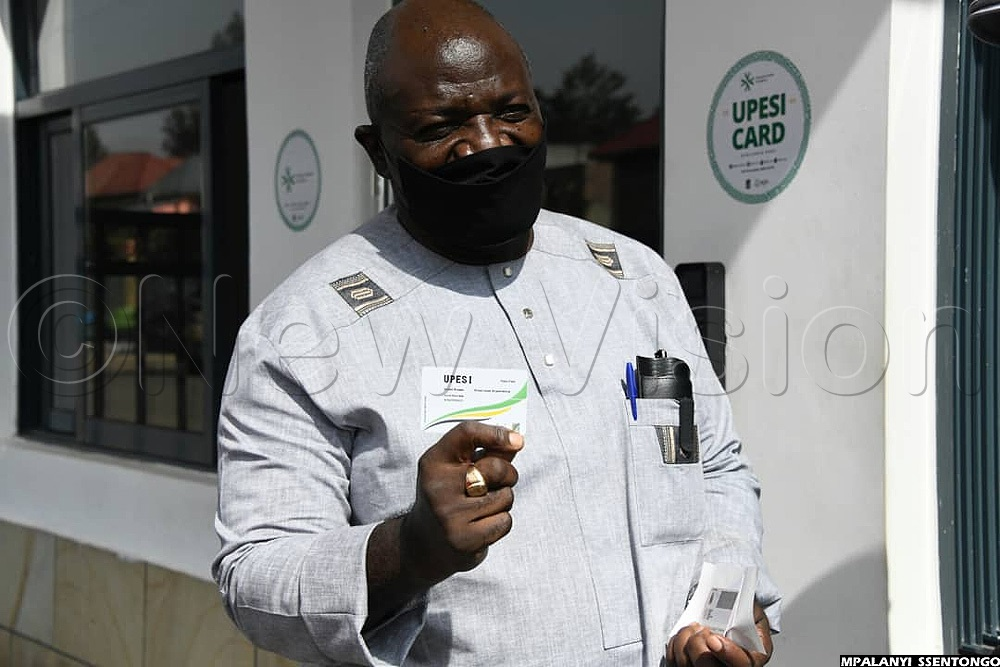
\includegraphics[scale = 0.3]{images/katus}
        \caption{Gen. Katumba Wamala showing an UPESI payment card on the launch of the Entebbe Express Highway}
    \end{center}
\end{figure}
The Uganda National Roads Authority in 2022 launched the Kampala Entebbe Express Highway, a  someting billion project to help ease transport flow in kampala. Access to the highway is via the toll gates where motorists can make both cash and digital  cashless payments. For cashless payments, motorists  use  an UPESI card.\cite{unra_news_2022}.  A motorist purchases an UPESI card that they then load a given amount of money and upon arrival at the toll gate, they swipe the card. The fee is then deducted from the card and the motorist is then granted access.

The main gap with the approach is motorists often resort to only using the cash payments that result in delays and other issues because they find it easier than purchasing an UPESI card. Additionally the process of loading money onto the card is unnecessarily long. Fine for losing card.

\subsection{ParkMobile}
Parkmobile is a leading mobile application launched in 2009 in the United States of America that allows motorists to find and pay for parking on their phone, and is currently used in approximately used in three thousand lcoations in North America. It also has over 43 million users and processed over 113 million parking transactions in 2022.
Parkmobile offers various features and benefits for its users, such as making prepayments and reserving parking points at any given location. It also offers a rewards program that allows users to earn points for every parking transaction and redeem them for discounts or free parking. Parkmobile also supports Google and Apple Pay for a faster and more secure payment process. \cite{parkmobile_2022}
The projeect has had good traction since it was launched and  in 2022 it generated $9.1 million in revenue , with an average revenue per employee of $52,906. Parkmobile was acquired by EasyPark Group, a Swedish company that provides smart parking and mobility solutions, in June 2021.

Unfortunately to the best of our knowledge, ParkMobile or any other application of this nature are not available in Uganda thus the need for a local contextualised solution

\subsection{Use of GPS Software and Cell Towers}
Research on how this can be leveraged in easing toll fee payment has been done by others. In 2020, Danang Dismantoro, Istas Pratomo and Surya Sumpeno also proposed a mobile application that allowed payment of these fees via GPS software\cite{el-rabbany_introduction_2002,dismantoro_minimizing_2020}. The system was tested through simulations in Vissim software \cite{ptv_vissim_traffic_2022}, which they believe was able to simulate the real world condition at tollgates. Cell phone towers and GPS technology are used to identify the motorist’ s location and if the motorist happens to be within the toll’s gate vicinity, the money is automatically deducted from their personal account.

\subsubsection{Research Gaps}
\begin{itemize}
    \item No physical implementation of this system was realised
    \item The researchers acknowledge the need for a deeper feasibility study and the fact as it has some shortcomings.
    \item Some scenarios are unaccounted for such as if one is near a cell tower but does not necessarily intend to access the tollgate,they’ll have their money deducted even without actually using the gate.
\end{itemize}

\subsection{Use of RFID sensors}
An RFID system has two main components:
\begin{itemize}
    \item A transponder: This is the tag that holds information, found on the object to be identified
    \item A reader/interrogator: This device is able to capture data from the tag.It has a radio frequency module,  control unit and coupling element for linking to the transponder. Additionally, an interface is added to pass on data captured from the transponder to a different system
\end{itemize}


Sabbir Ahmed et al in 2019 also proposed a similar solution.Their proposed system would simplify toll payment through use of RFID tags placed on digitised license plates of all vehicles.Once the tag is scanned, and the motorist has a sufficient balance on their account, the vehicle is granted access\cite{ahmed_automated_2019}.


Another study by Etqad Khan et al. in 2018 proposed a system similar to ours that would ease payment of toll fees using RFID tag that would be linked to motorists' personal accounts where would have a mobile e-wallet on which a given amount would be saved.The system also provides a mobile application to view their past payments\cite{khan_automated_2018}.

\begin{figure}
    \begin{center}
        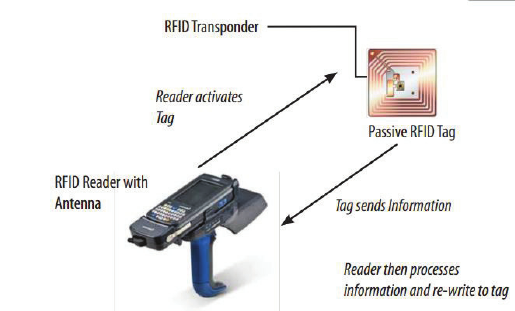
\includegraphics[scale = 0.3]{images/rfid-pic}
        \caption{Components of an RFID system}
    \end{center}
\end{figure}

\subsubsection{Research Gap}
These two identified studies are constrained in our project scope’s context, because:
\begin{itemize}
    \item It would first off require digitisation of all vehicle license plate, an endeavour that has not yet been taken on by the government of Uganda.
    \item Long range RFID tags and scanners are costly to purchase which would be needed in this use case are costly ,and would thus the need for a low-cost solution that’s accessible to majority of the motorists.
\end{itemize}



\clearpage


\section{Our Contribution}
Alot of work has been done by other researchers to address the issue of tollgate queues. Many of these solutions leverage RFID technology as an alternative to the physical cash payments. This would however require purchasing costly scanners and tags, thus the need for a similar but cheaper solution.
The biggest benefits to our proposed system:
\begin{itemize}
    \item Developing a low-cost and context-specific solution for cashless parking payment using local popular payment platforms such as MTN mobile money
    \item Designing and implementing a mobile app and an embedded microcontroller that interact using QR codes to facilitate parking access and payment
    \item Evaluating the performance and usability of the system and comparing it with the current system of ticketing and payment
    \item Examining the benefits and challenges of the system, such as security, scalability, and user acceptance
    \item Providing insights and recommendations for improving parking management in the university context and in developing countries in general
\end{itemize}

\begin{figure}
    \begin{center}
        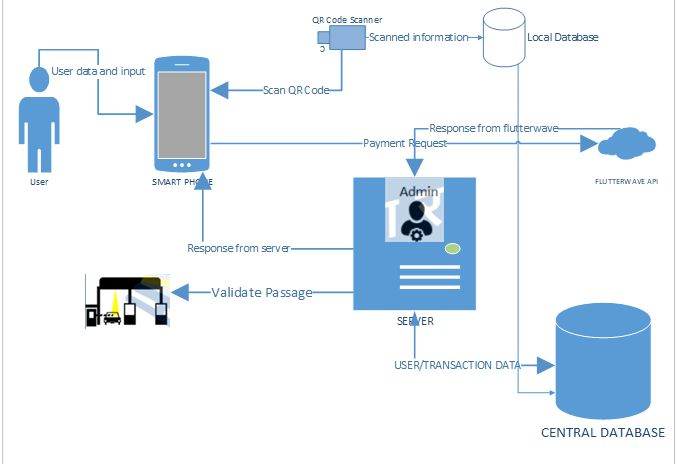
\includegraphics[scale = 0.6]{images/etolssys}
        \caption{System Architecture Diagram for the proposed solution }
    \end{center}
\end{figure}


    \chapter{Methodology}\label{ch:methodology}
    \section{Introduction}
This chapter discusses the techniques that were used to achieve the objective of the proposal. It covers the approaches used for data collection, design, final implementation, and system testing. The results from the data gathering and other steps of our methodology are presented and discussed in the next chapter.


\section{Data Gathering and Elicitation}
The team collected relevant and appropriate data to determine the requirements of the proposed system. This was done through questionnaires, interviews and physical observation\cite{kothari_research_2004}.

\subsection{Questionnaires}
Questionnaires contain open or closed ended questions given to a selection respondents to solicit information on a selected research topic\cite{bartram_using_2019}. Google forms \cite{googleforms} were be used to create online questionnaires that were shared through social media and emails to targeted stakeholders. Advantages of online questionnaires are that they are relatively easy and quick to distribute. It is also quicker to receive responses and the data can be collected directly for analysis. The survey questions for this research are available in the report appendix. The questionnaires were distributed to a total of 52 respondents from various categories of users of the current system. Details on the respondents are shown discussed in the next chapter on System Analsysis and Design.

\subsection{Interviews}
An interview is a one on one planned conversation with a person with an aim of attaining information. Researchers had interactions with owners of the system currently in place as well as a selection of the motorists in order to get firsthand information on issues faced. This helped us in better defining the system requirements of the project. The interviews also enabled the researchers to establish relationship with potential respondents as well as owners of the current system and therefore gain their corporation,  yielding highest response rates in the survey research. The researchers conducted 2 interviews with Mr. Twinomusinguzi Julius the project manager of the current system in place, and from these we were able to better understand the current system and its challenges. The interview questions are available in the report appendix.

\subsection{Observation}
Observation involves spending time with stakeholders and keenly monitoring their activities. Researchers took a physically closer look at what takes place during the daily activities of motorists trying to access the university and the challenges they face and will entail systematic noting and monitoring of events, behaviors of the motorists as they go on with their activities.


\section{Data Analysis}
This was done to remove inconsistencies in the data collected, as well as sieve out useful data that will be used to improve the system requirements.


\section{System Design}
For the system design, context diagrams were created and used to define the scope of the project and its environment as well as the entities who will interact with it.Additionally, there were detailed processes of how the system works. \cite{rumbaugh_object-oriented_1991}.

\subsection{Process Modelling}
Here, data flow diagrams were used to demonstrate the processes and entities that interact with the system.

\subsection{Data Modelling}
Entity relationship modelling was done to identify the entities as well as their relationship how they interact with each other.
This was achieved by use modelling entity relationships. The researchers used a top down approach to identify the entities interacting with the system.


\section{System Implementation}
At this stage the team built the E-Tolls application.A number of tools and technologies were used and these are defined below:

\subsection{Software tools}
\begin{itemize}
    \item  Android Studio \& Xcode: This is where the mobile application was developed.
    \item Arduino IDE: This was used to write the code for the microcontroller.
    \item Flutter mobile framework: This will be used to write the cross-platform code for the application
    \item DigitalOcean: This will be used to host the remote server.
    \item Silicon Pay: This will be used to process payments which are computed dynamically basing on the time one has spent within the premises
\end{itemize}

\subsection{Hardware tools}
\begin{itemize}
    \item ESP32 microcontroller
    \item Servo motor to demonstrate the opening and closing of the gate
    \item Camera to be used to scan QR codes
    \item Wi-FI GSM module to enable internet connection of the microcontroller
    \item FTDI connector to enable connection of the microcontroller to the computer
\end{itemize}


\section{System Testing and Validation}
Here,  the system is deployed and executed to assess its functionality. The system was deployed on a server and released as a prototype for user testing and validation. The purpose of validation was to ensure that the system performs precisely as intended in a consistent and efficient manner.

To validate the system, various methods were employed, including testing the prototype with invalid data and assessing how it handles exceptions. The android application was deployed to Firebase app distribution and shared with selected internal testers to try out and share feedback on the application. The feedback was used to improve the application and fix any existing issues.


\section{Conclusion}
In conclusion, this chapter has outlined the procedures followed in the creation of the E-Tolls Mobile Application. The system we believe will be able to meet not just the requirements of the users but also the objectives of the project.


    \chapter{System Analysis and Design}\label{ch:system-analysis-and-design}
    \section{Overview of the System}
This chapter consists of the general introduction, the study of the existing system, requirement specification and system design. The study of the existing system includes main findings from interviews, requirements specifications include functional, non-functional requirements, software and hardware requirements. System design comprises modelling the solution basing on findings from the interviews.


\section{System study}
The data gathered using the selected data collection techniques enabled the system developers to garner information which was studied to realise the weaknesses of the existing systems and how the new system would be designed in a better way.


\section{Study of the existing system}
Our case study as previously mentioned was the Makerere University Parking System. We conducted two interviews with the project manager who informed us all the details of the current system and its shortcomings. Some details however such as average revenue garnered by the system,etc. were not shared with us for confidentiality purposes.


\section{System Analysis}

\subsection{Data Analysis}
Below is a summary of some of the main findings from the survey we conducted.

\subsubsection{Breakdown of the users of the existing and proposed system}
Our analysis found that the main users of the system are fall into two categories, each with its own subcategories. These are:
\begin{itemize}
    \item Frequent users: This comprises users students, lecturers and university staff who are the main users of the system.
    \item Occasional users: This comprises visitors to the university or ordinary passers-by who wish to use the system quickly perhaps a shortcut to avoid traffic, or a brief visit to the university, among other reasons
\end{itemize}
The system therefore ought to have a way to discern between these two categories, and frequent users are not expected to make payments every time they use the system. To achieve this, registered users can register with their student or university credentials, and the system can then verify their status and allow them to use the system without making payments. The occasional users can then be charged for each use of the system.



\begin{figure}[h]
    \hspace{-1cm}
    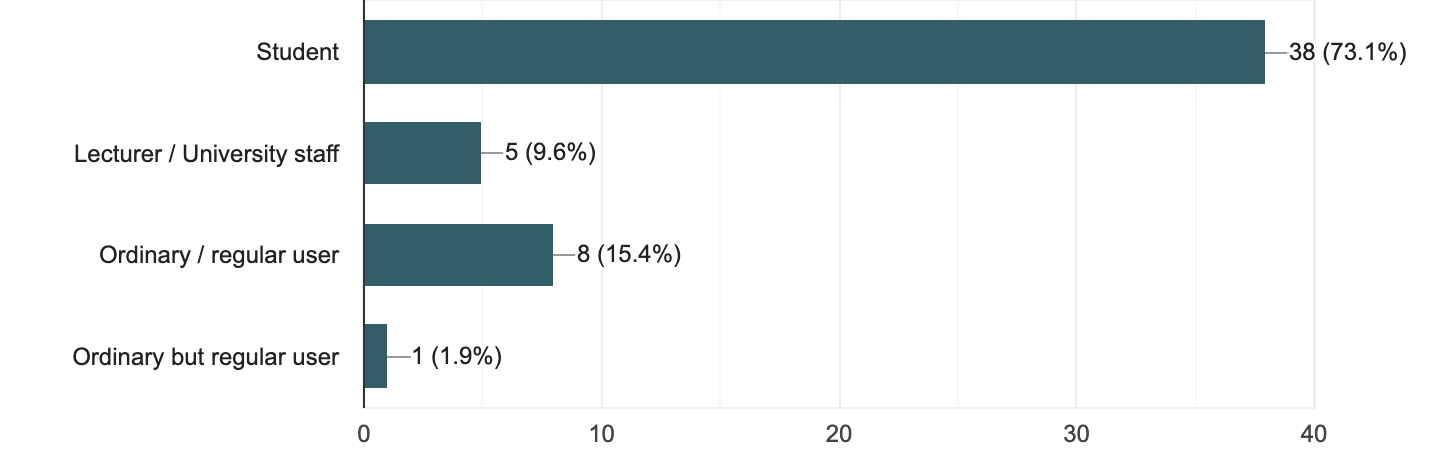
\includegraphics[scale = 0.5]{images/users}
    \caption{Breakdown of intended users of the system}
\end{figure}

\clearpage

\subsubsection{Analysis of frequency of usage of the current system}
We were also able to analyse the frequency of usage of the current system. We found that the majority of our respondents use the system on a daily basis, with a few using it on a weekly basis. This is expected since the main users of the system are students, lecturers and university staff who are expected to be at the university on a daily basis. The occasional users are expected to be a minority.


\begin{figure}[h]
    \begin{center}
        \hspace{-1cm}
        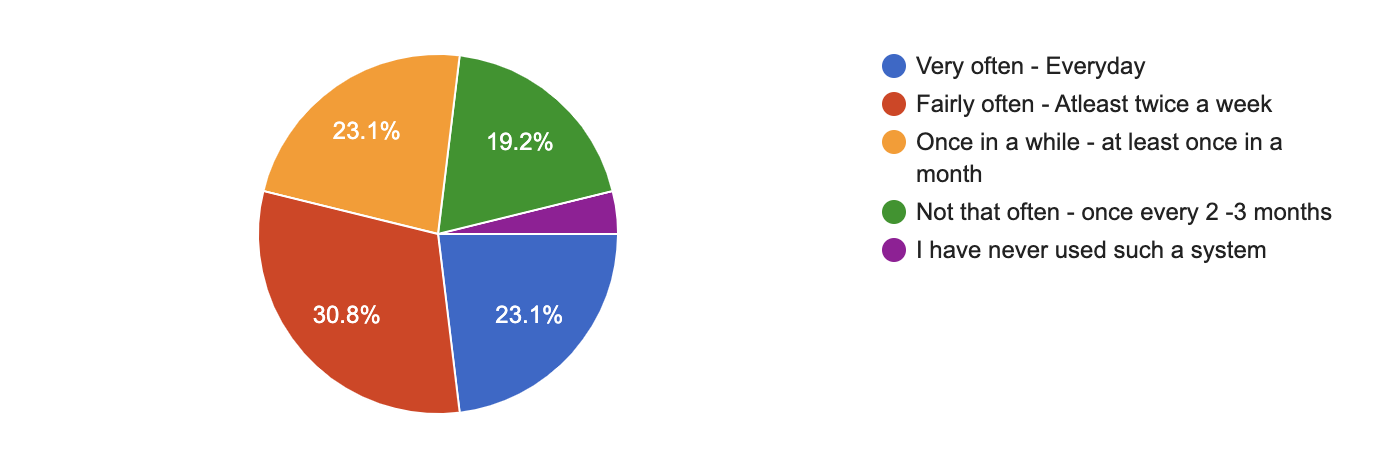
\includegraphics[scale = 0.5]{images/usage}
        \caption{Respondents' frequency of usage of the current system}
    \end{center}
\end{figure}

\clearpage

\subsubsection{Familiarity with local mobile payment platforms}
We believe one of the benefits of our proposed system is that we leverage local mobile money platforms such as MTN Mobile Money and Airtel Money. We therefore sought to find out how familiar our respondents were with these platforms. We found that the majority of our respondents were familiar with these platforms, with a few not being familiar with them. This is expected since mobile money is a popular payment platform in Uganda.


\begin{figure}[h]
    \begin{center}
        \hspace{-1cm}
        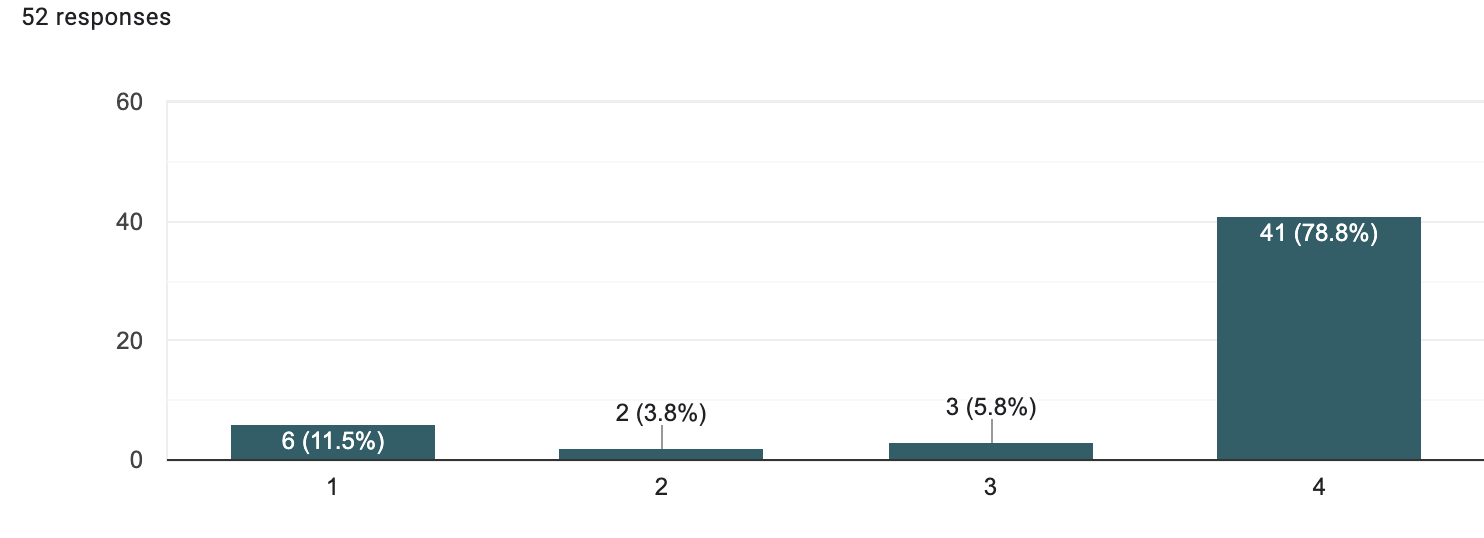
\includegraphics[scale = 0.5]{images/mob-mon}
        \caption{Respondents' familiarity with mobile money platforms on a scale of 1 to 5}
    \end{center}
\end{figure}

\clearpage

\subsubsection{Level of satisfaction with existing system}

We also sought to find out how satisfied our respondents were with the existing system. We found that the majority of our respondents were either not satisfied or fairly satisfied with the existing system, with a few being satisfied with it. This is expected since the existing system has a number of shortcomings which we have already highlighted.

\begin{figure}[h]
    \begin{center}
        \hspace{-3cm}
        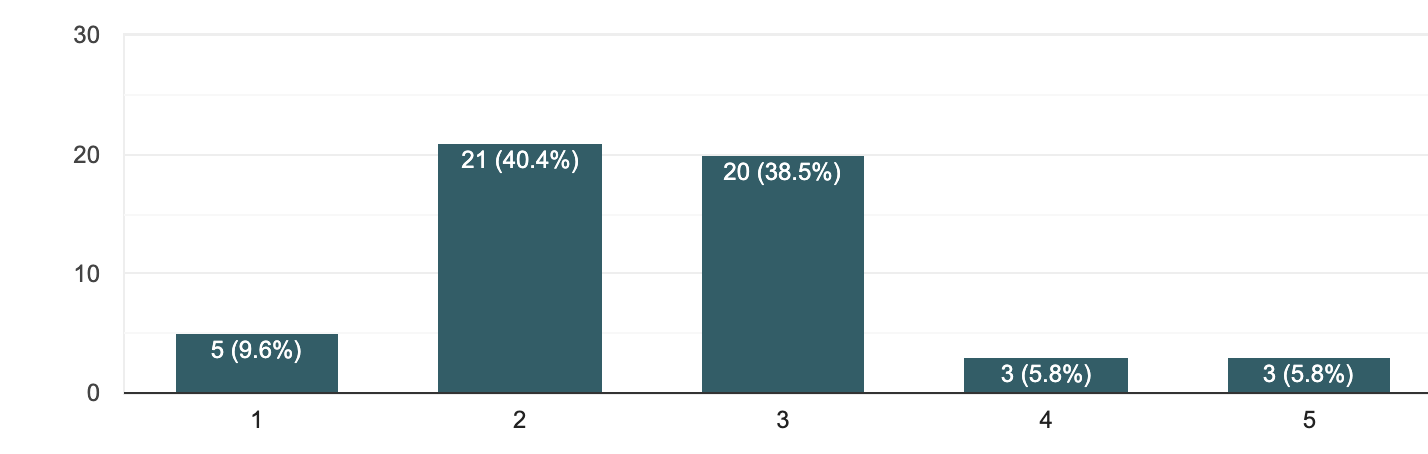
\includegraphics[scale = 0.5]{images/satisfaction}
        \caption{Respondents' level of satisfaction with the existing system on a scale of 1 to 5}
    \end{center}
\end{figure}

\clearpage

\subsubsection{Frequency of encountering challenges with the existing system}
We also sought to find out how often our respondents experienced problems such as malfunction of the ticketing machine, difficulty finding the payment points. We found that the majority of our respondents experienced problems with the existing system occasionally, others frequently and a few never experienced problems with the existing system.

\begin{figure}[h]
    \begin{center}
        \hspace{-3cm}
        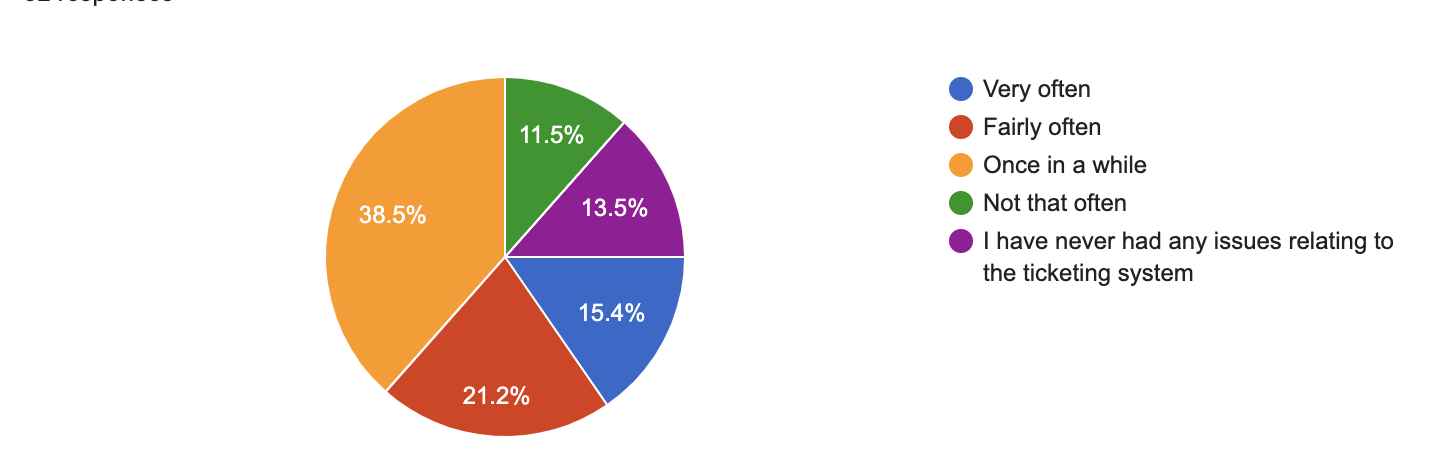
\includegraphics[scale = 0.6]{images/prob-freq}
        \caption{Respondents' frequency of encountering problems with the existing system}
    \end{center}
\end{figure}

\subsubsection{Opinion on the hefty fine for losing a ticket}
The researchers also sought from the respondents their individual opinions on the hefty fine for losing a ticket. All respondents expressed dissatisfaction with the idea, justifying the need for a digital alternative of ticketing that avoid such scenarios.


The interview guide used during the interview with the project manager as well as survery questions are attached in the appendix.
\clearpage

\subsection{Requirements Specification}
In order to come up with the end user requirements for the new system, data was collected through interviews with both the project manager of the current system at Makerere University and a survey shared with motorists who use the gates.

The collected data was then analysed in order to come up with the requirements of the new system. This section included the requirements of the new system divided into user requirements and system requirements.

\subsubsection{User Requirements}
This encompasses the requirements of the system from the user’s point of view.

The users identified are gate attendants who can also double as administrators of the system as well as motorists who use the gates. The motorists are split into two further categories: regular users and occasional users.
\begin{itemize}
    \item \textbf{Gate attendants / Administrators}: Manages the ETolls System
    \item \textbf{Motorists}: Uses the ETolls System to make their payment
\end{itemize}

\subsubsection{Functional Requirements}
This is to with the services that the system will provide to the users. The system will be able to:
\begin{itemize}
    \item Allow new users(motorists) to register for the system
    \item Allow registered users to log in to the system
    \item Allow users to make payments for parking
    \item Allow users to view their payment history
    \item Allow users to view their parking history
    \item Allow the system administrator to add or delete users
\end{itemize}

\subsubsection{Non-Functional Requirements}
These are requirements that are not directly related to the functionality of the system but are important for the system to work properly. These include:
\begin{itemize}
    \item The system should allow for easy registration of users
    \item The system should support various payment platforms such as MTN Mobile Money, Airtel Money
    \item The system should be secure
    \item The system verifies all user inputs and users must be notified in case of error
\end{itemize}

\subsection{System Design}
This section defines the physical architectural design and the logical design (showing processes, sub processes and entties)  of the system required to satisfy the specified requirements.

\subsubsection{Architectural Design}
An architecture diagram is a representation of elements that comprise a given system\cite{tilley2019systems}.

The system will comprise a mobile application as well as remote server hosted on the cloud. The mobile application will be used by the motorists to make payments and view their payment history. The remote server will be used to store the data of the users and their payment history. The final component is the microcontroller which will be used to control the gates and communicate with the remote server.

For demonstration purposes, the system will be demonstrated using a microcontroller and a servo motor to demonstrate the logic of opening and closing of gates


\begin{figure}[h]
    \begin{center}
        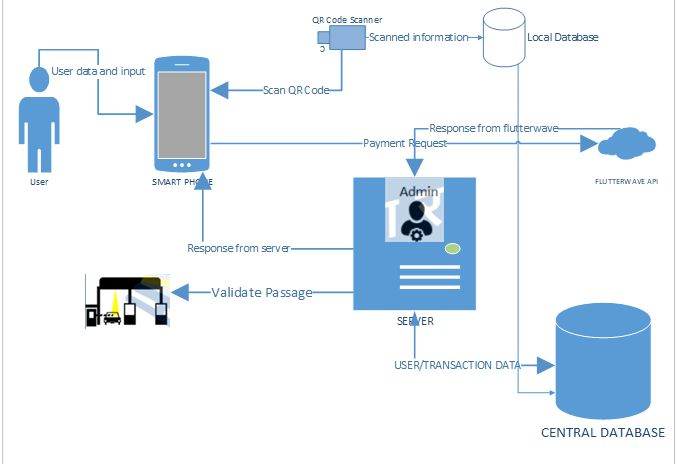
\includegraphics[scale = 0.8]{images/etolssys}
        \caption{System Architecture diagram for E-Tolls System}
    \end{center}
\end{figure}

\clearpage

\clearpage

\subsubsection{Use case diagram}
A use case diagram is a graphical representation of a given user's possible interactions with a system. It gives broad view of a system and the different types of users and use cases within that system \cite{alhir2003learning}.
Below is a use case diagram for our proposed system
\begin{figure}[h]
    \begin{center}
        \hspace{-0.6cm}
        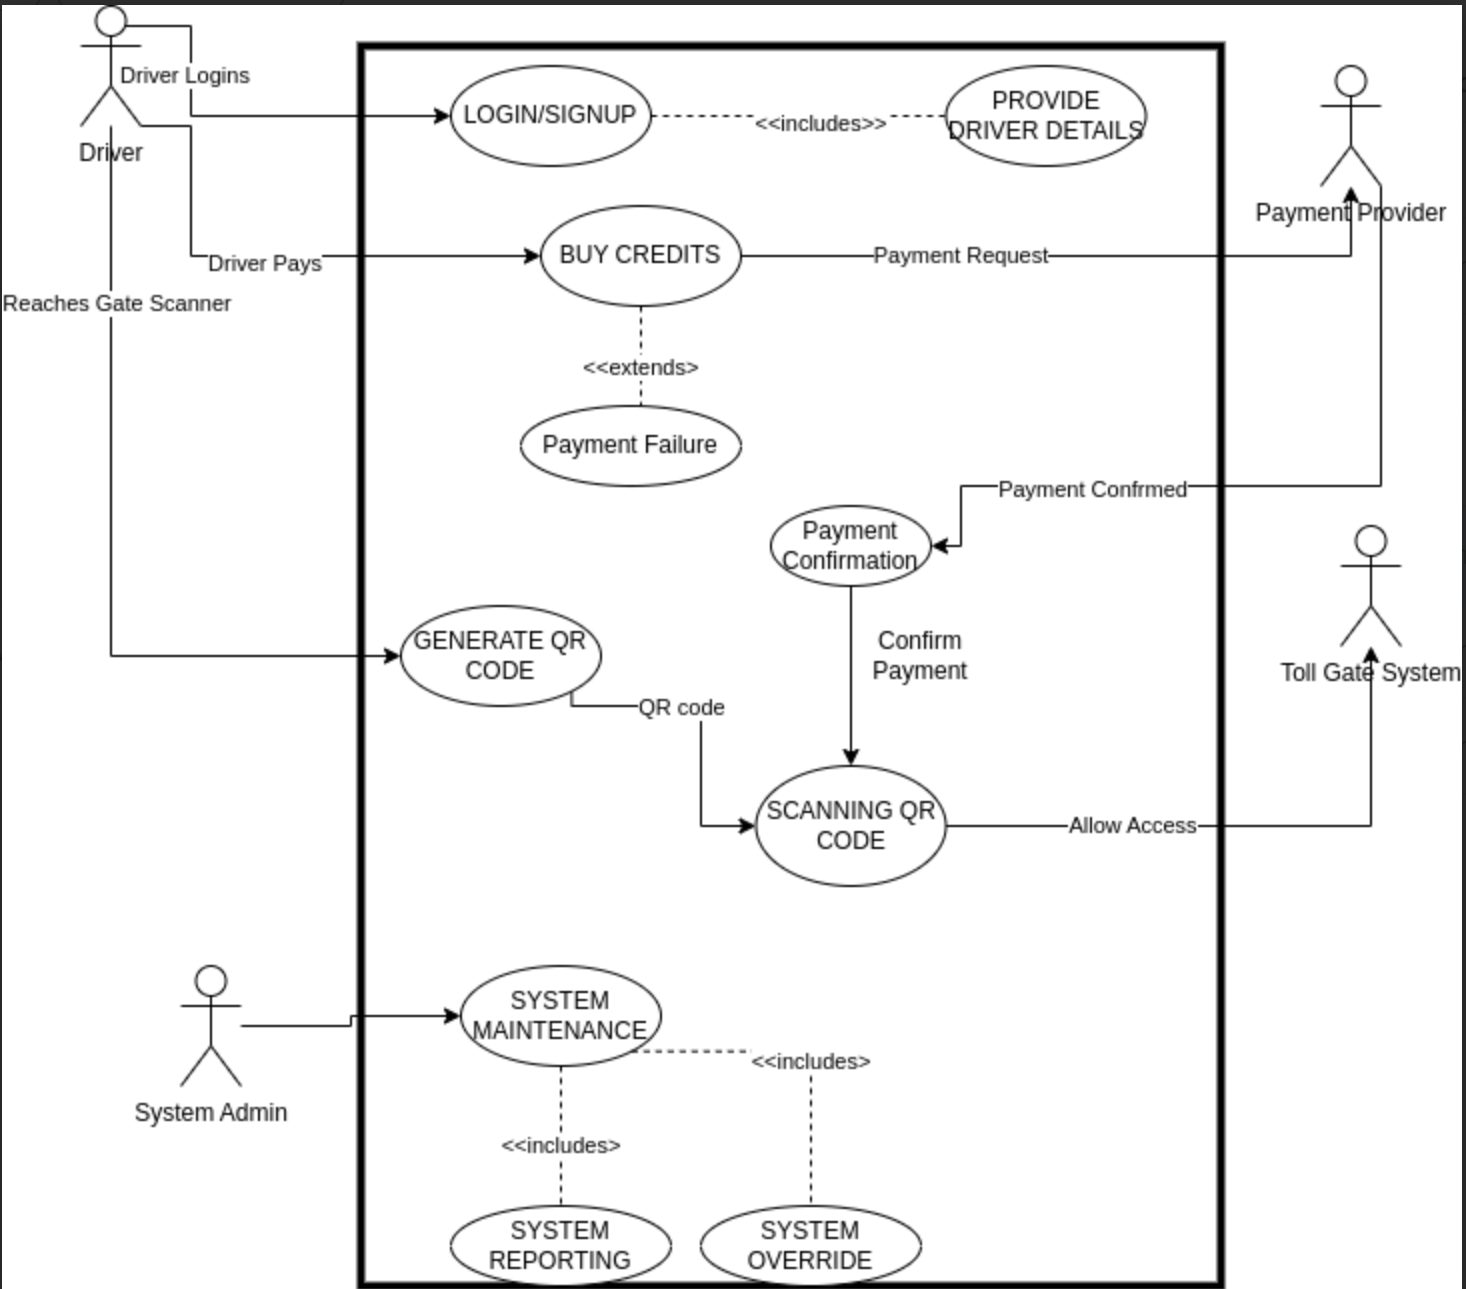
\includegraphics[scale = 0.45]{images/use case diagram}
        \caption{Use Case diagram for E-Tolls System}
    \end{center}
\end{figure}

\clearpage

\subsubsection{Entity Relationship Diagram}
An entity relationship diagram (ERD), also known as an entity relationship model, is a graphical representation that depicts relationships among people, objects, places, concepts or events within a system. The diagram below shows the entities and their relationships in our system\cite{bagui2012database}.
\begin{figure}[h]
    \begin{center}
        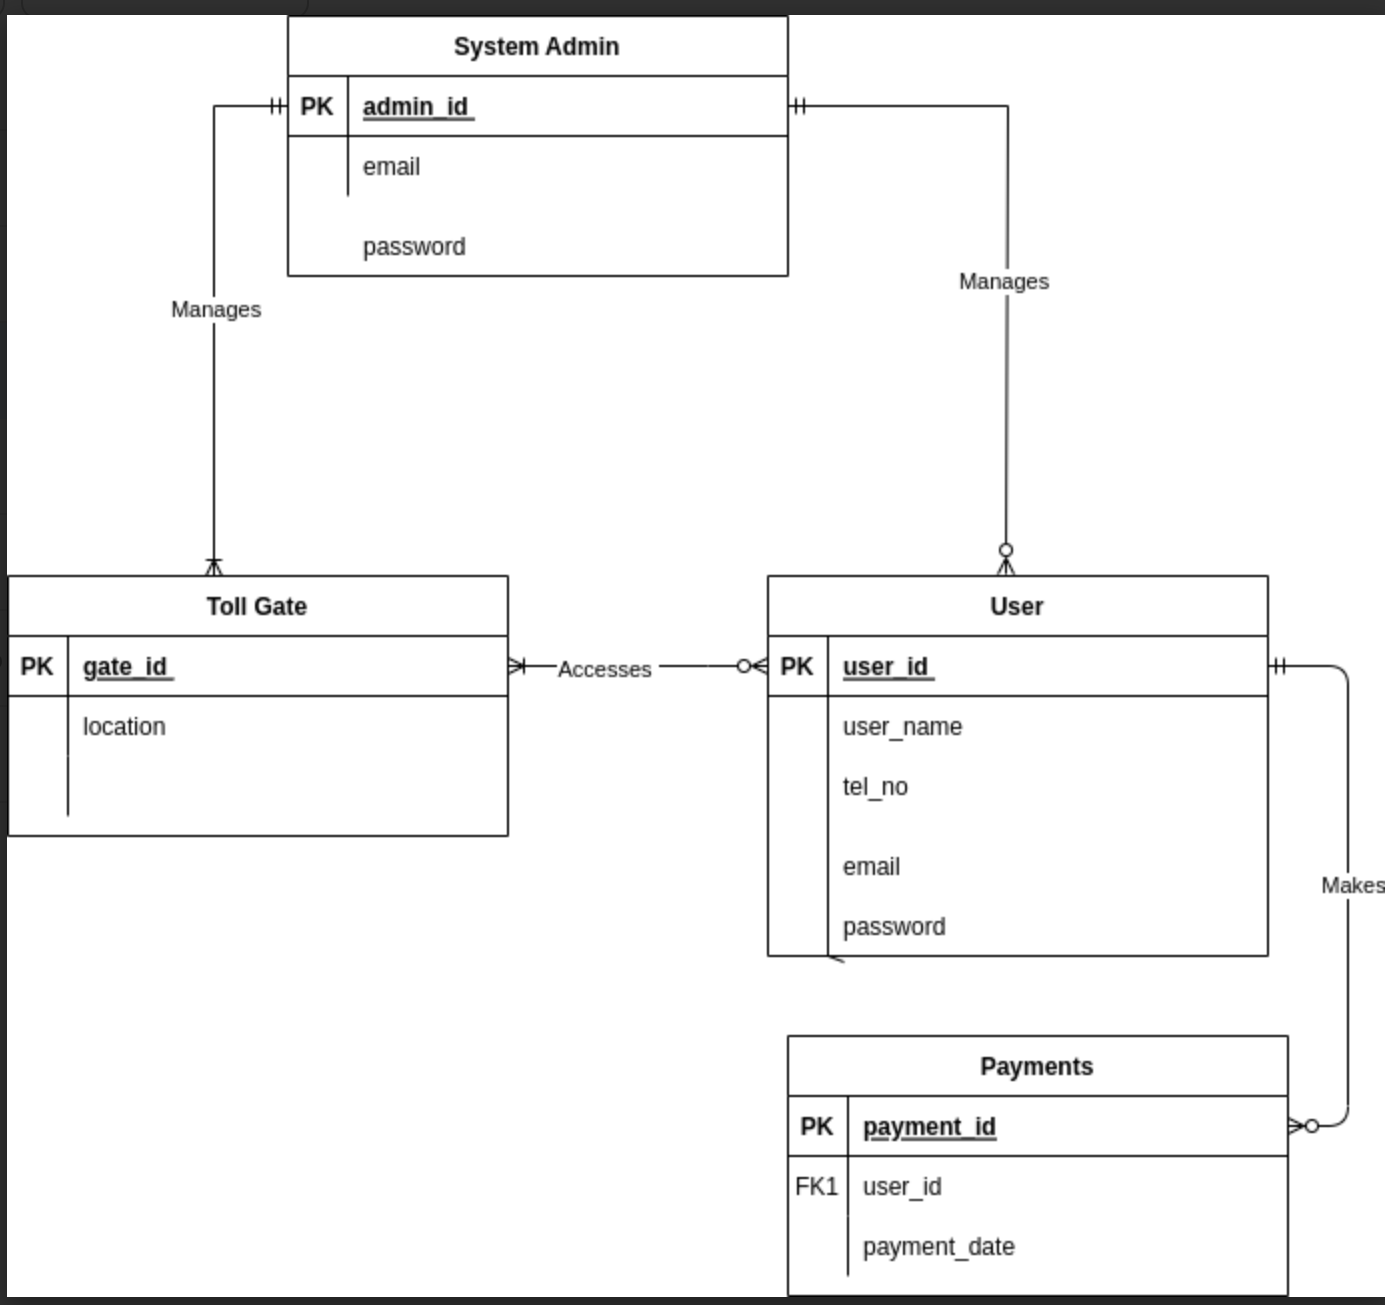
\includegraphics[scale = 0.45]{images/erd}
        \caption{Entity Relationship Diagram for E-Tolls System}
    \end{center}
\end{figure}


\clearpage

\subsubsection{Flow chart}
The flow chart represents the dynamic behavior of the objects and classes that have been identified as part of the system. The flow chart helped us describe the plan in order to perform the different tasks. It showed what was done when the decision was made and when to go to each process as a result. The flow chart helped us build a step-by-step picture of the processes of our system.
\begin{figure}[h]
    \begin{center}
        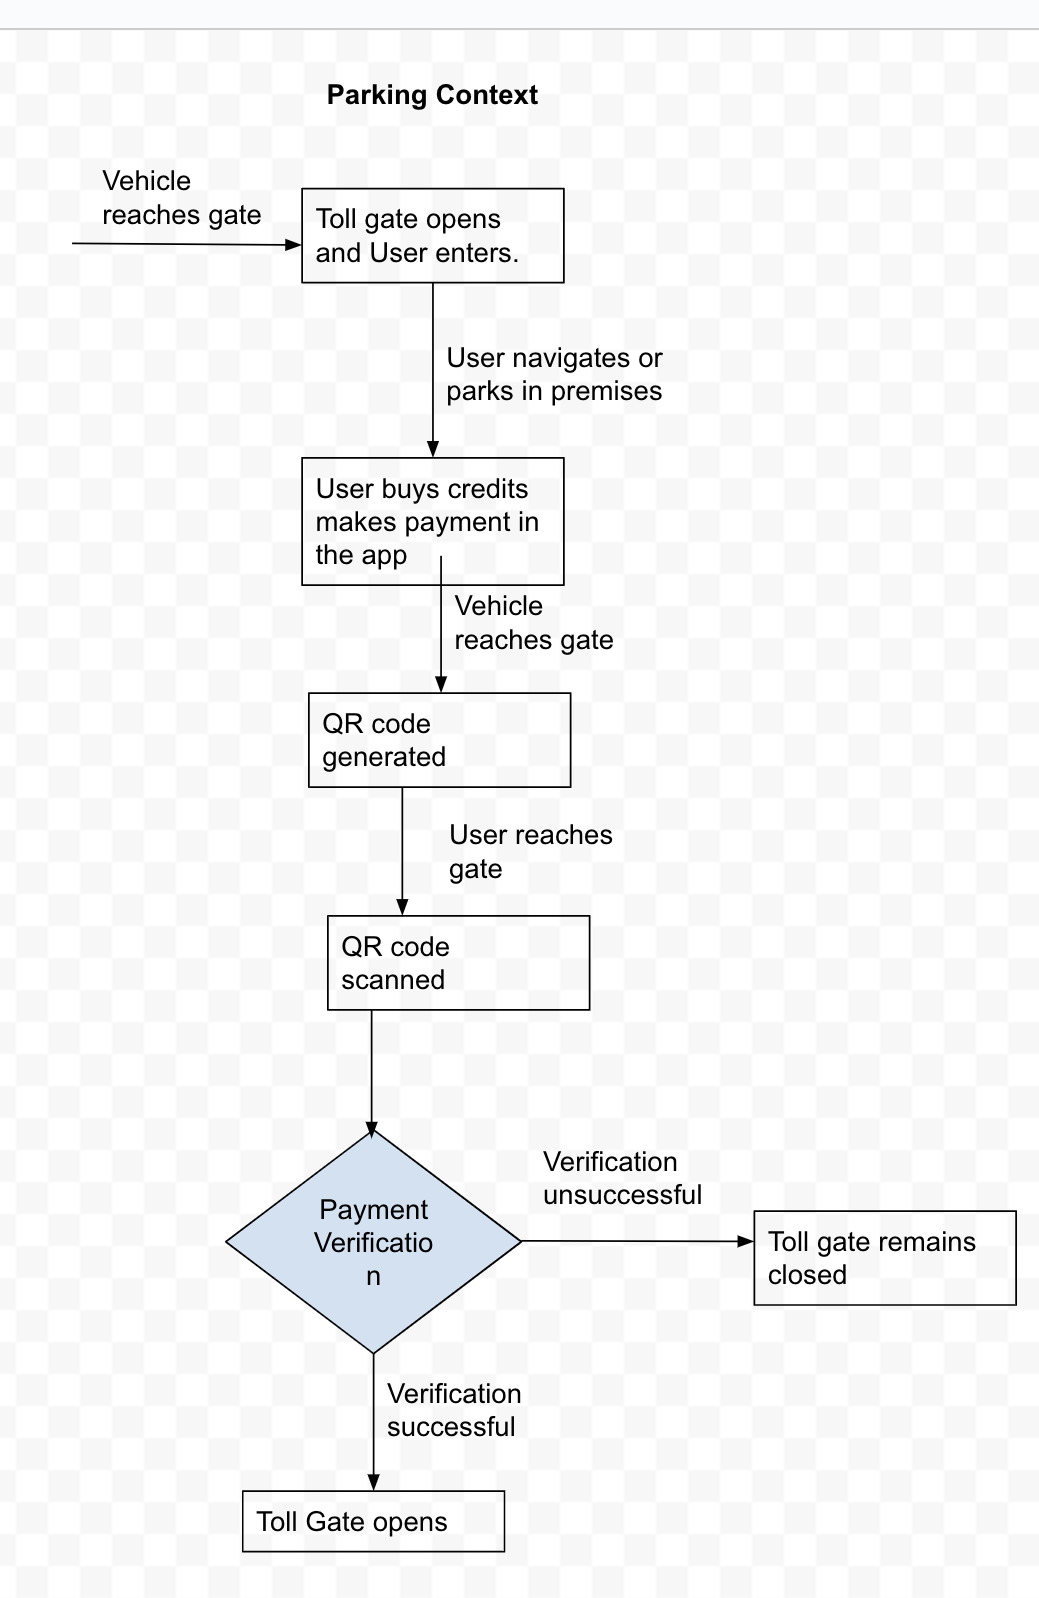
\includegraphics[scale = 0.6]{images/userflowdiagram}
        \caption{System Architecture diagram for E-Tolls System}
    \end{center}
\end{figure}
\clearpage

\subsubsection{Context Diagram}
A context diagram provides a visual representation of how external elements interact with a system, such as a project or a software system. It clarifies the interfaces and boundaries of the project or process at hand, and shows the project’s interactions with other systems and users\cite{wysocki2006effective}.

\begin{figure}[h]
    \begin{center}
        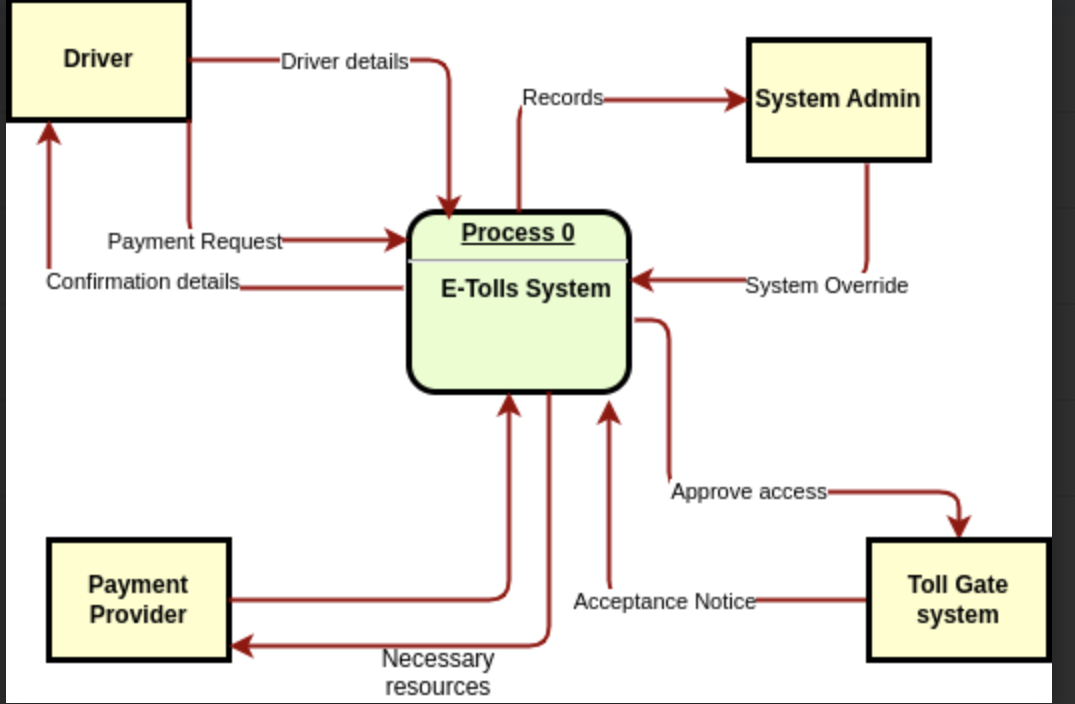
\includegraphics[scale = 0.6]{images/context_diagram}
        \caption{Context Diagram for E-Tolls System}
    \end{center}
\end{figure}


    \chapter{Presentation of Results}\label{ch:results-presentation}
    \section{Introduction}\label{sec:introduction}
This chapter shows screenshots of the system interface, connections of the hardware equipment and other details the programming environment that was used to develop the system.


\section{Implementing the system}

\subsection{Programming Tools}
The system was implemented using the following programming tools:
\begin{itemize}
    \item \textbf{Android Studio}: This is the official IDE for Android development. It was used in the development of the mobile application.
    \item \textbf{Arduino IDE}: This is the official IDE for Arduino development. It was used in the development of the microcontroller code.
    \item \textbf{Digital Ocean}: This is a cloud hosting service. It was used to host the remote server.
    \item \textbf{Flutter}: This is a cross-platform UI toolkit developed by Google. It is used to develop the mobile application.
    \item \textbf{Firebase}: This is a mobile and web application development platform developed by Google. It is used to handle user authentication.
    \item \textbf{Silicon Pay}: This is the payment gateway the researchers opted for due to its support for all local payment platforms
    \item \textbf{ESP32 Microcontroller}: This is a microcontroller developed by Espressif Systems. It is used to receive data from the mobile application and send it to the remote server.
    \item \textbf{Servo Motor}: This consists of a DC motor, gearbox, and a control circuit. It has a simple lever that can be attached to it and used to demonstrate the opening and closing of the gate upon verification of payment.
    \item \textbf{FTDI connector}: This is a USB to serial adapter that is used to program the ESP32 microcontroller.
\end{itemize}

\clearpage

\subsection{Embedded Systems Equipment}
The following equipment was used in the development of the system:
\begin{figure}[h]%
    \centering
    \subfloat[\centering]{{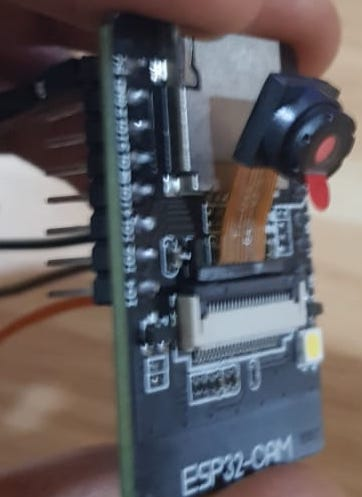
\includegraphics[scale=0.32]{images/esp1} }}%
    \qquad
    \subfloat[\centering]{{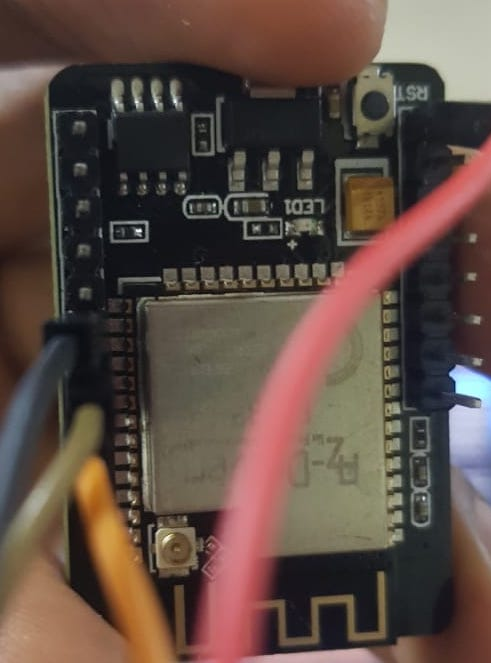
\includegraphics[scale=0.24]{images/esp2} }}%
    \caption{ESP32 microntroller used to scan the user QR codes}%
    \label{fig:equip}%
\end{figure}
\begin{figure}[h]
    \centering
    \subfloat[\centering]{{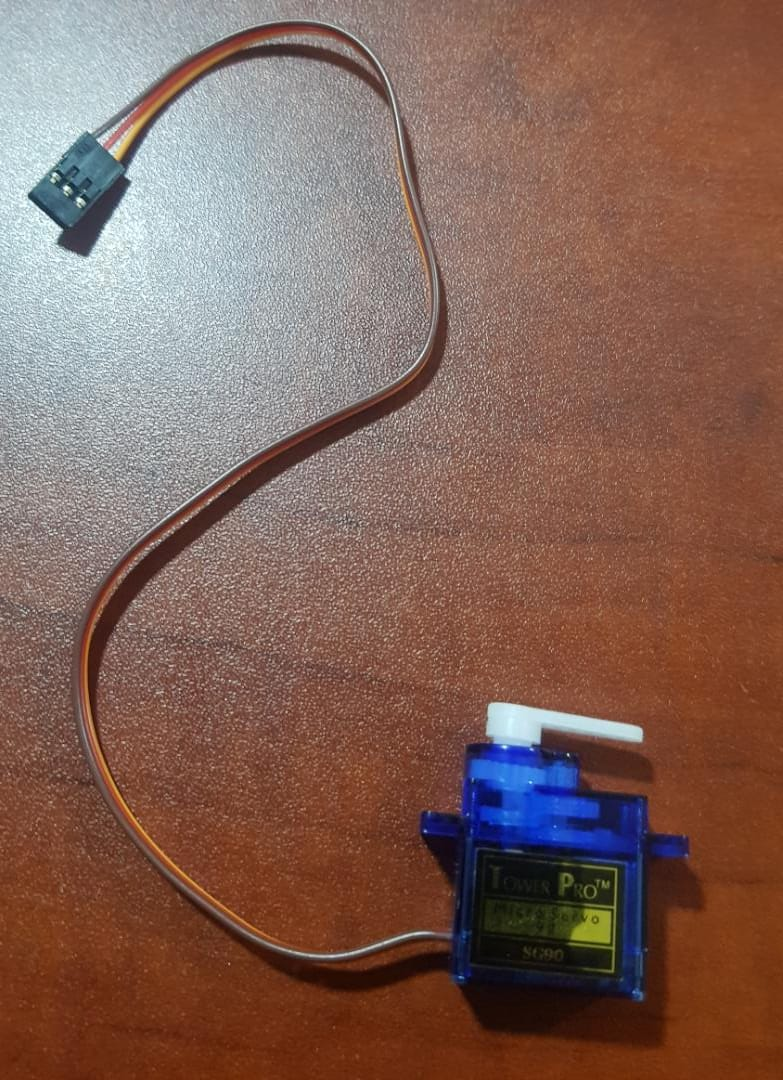
\includegraphics[scale=0.12]{images/servo} }}%
    \qquad
    \subfloat[\centering]{{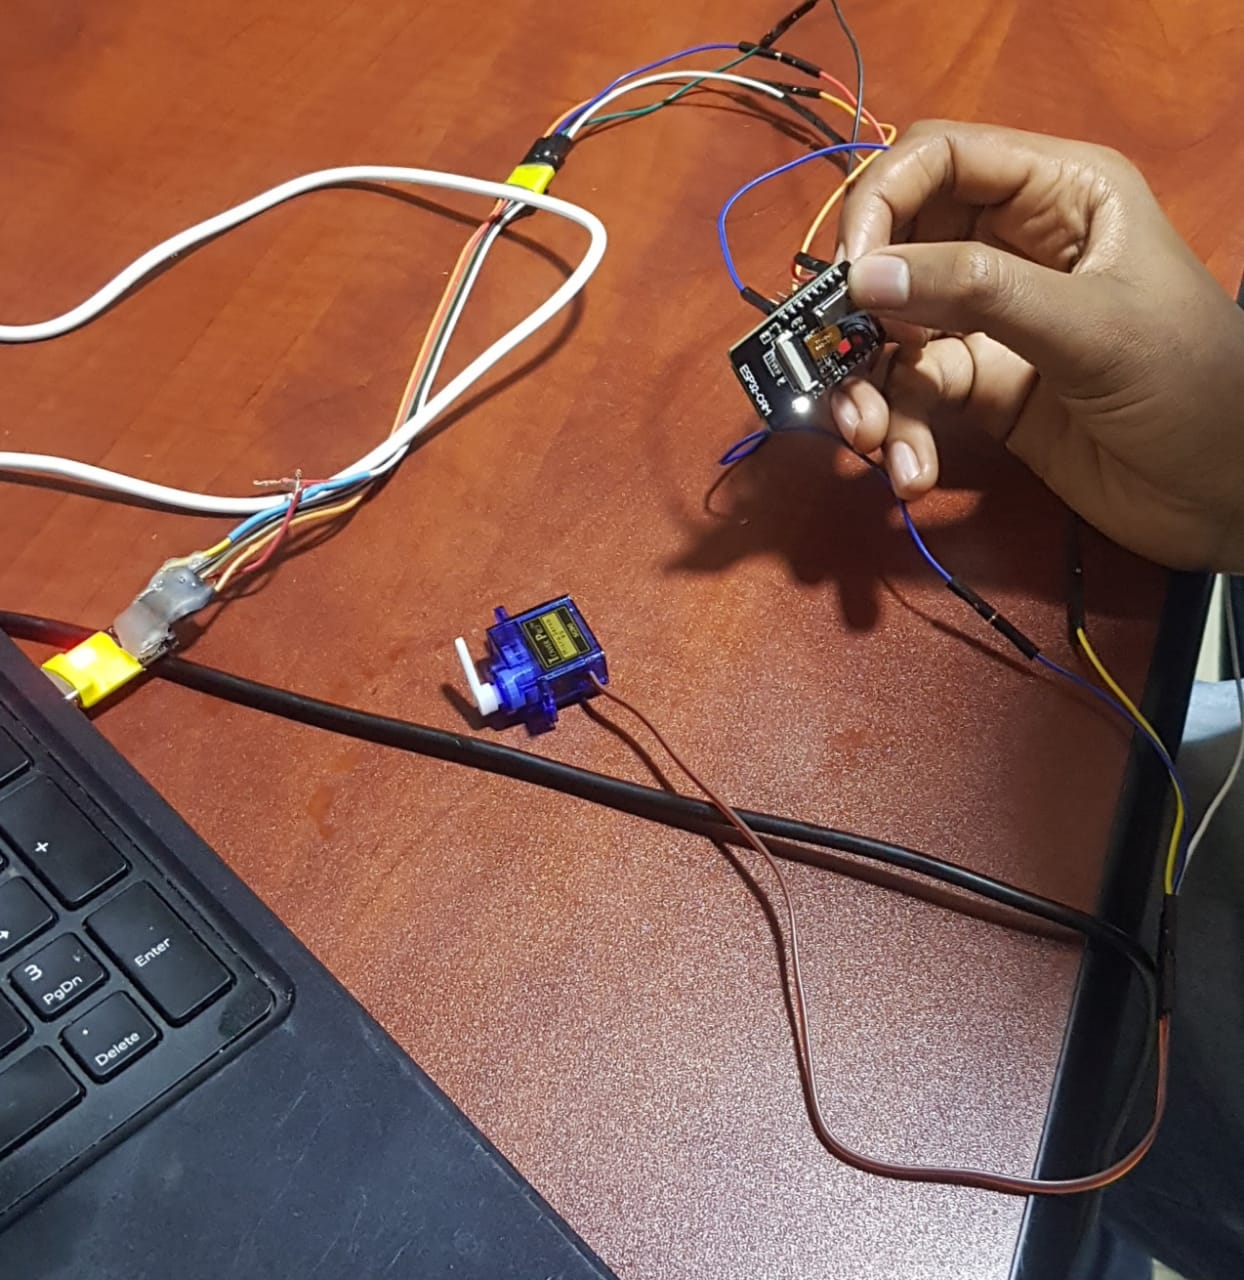
\includegraphics[scale=0.1]{images/full-connection} }}%
    \caption{Left is a servo motor used to demonstrate closing and opening logic and Right is the complete connection of the equipment }%
    \label{fig:equip}%
\end{figure}
\clearpage

\subsection{Screenshots of the mobile application in order of use}
\begin{figure}[h]%
    \centering
    \subfloat[\centering]{{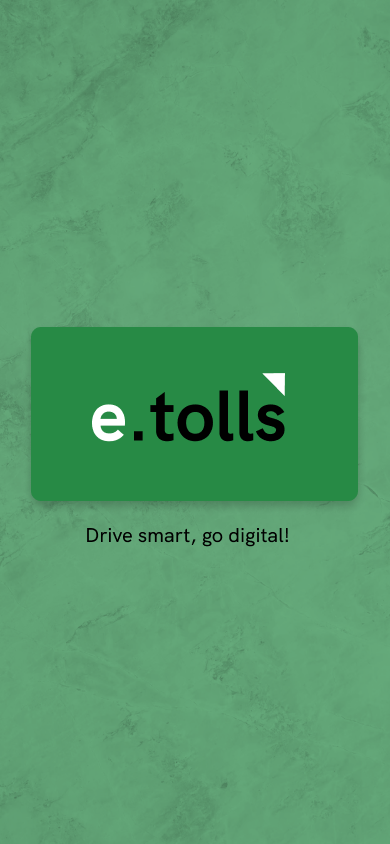
\includegraphics[scale=0.17]{images/Splashscreen} }}%
    \subfloat[\centering]{{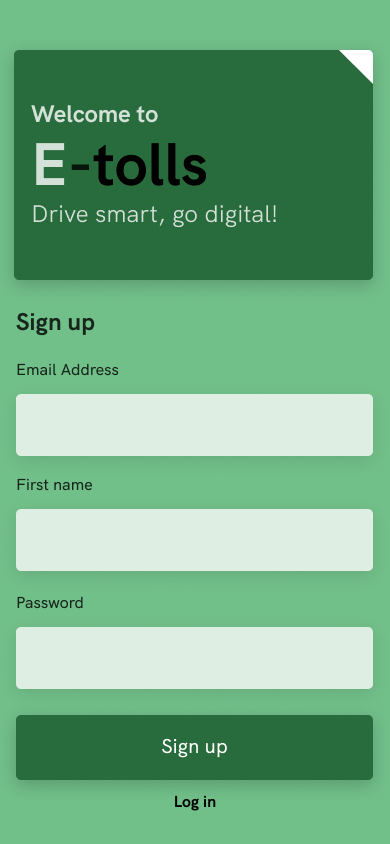
\includegraphics[scale=0.17]{images/Signup} }}  \subfloat[\centering]{{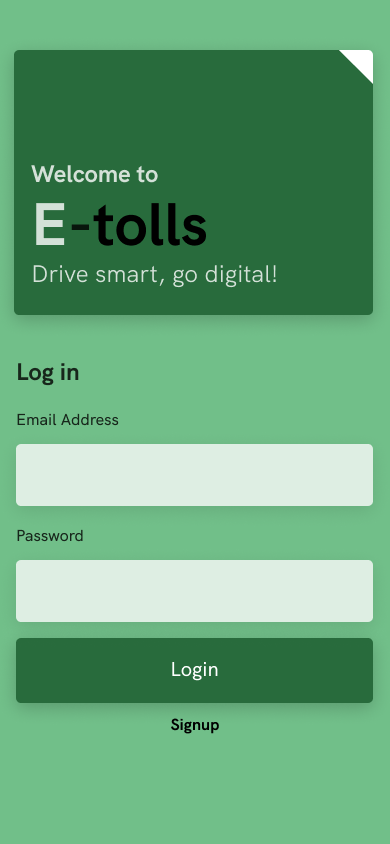
\includegraphics[scale=0.17]{images/Log in} }}%
    \caption{Login and Sign Up Screens of the mobile application}%
    \label{fig:example}%
\end{figure}
\begin{figure}[h]%
    \centering
    \subfloat[\centering]{{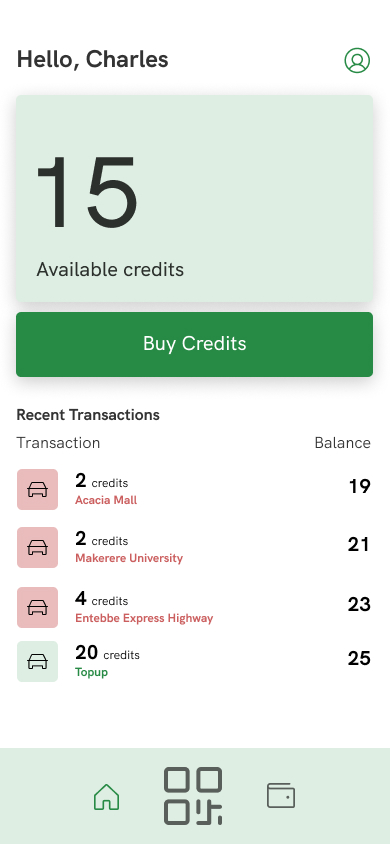
\includegraphics[scale=0.17]{images/Home} }}%
    \subfloat[\centering]{{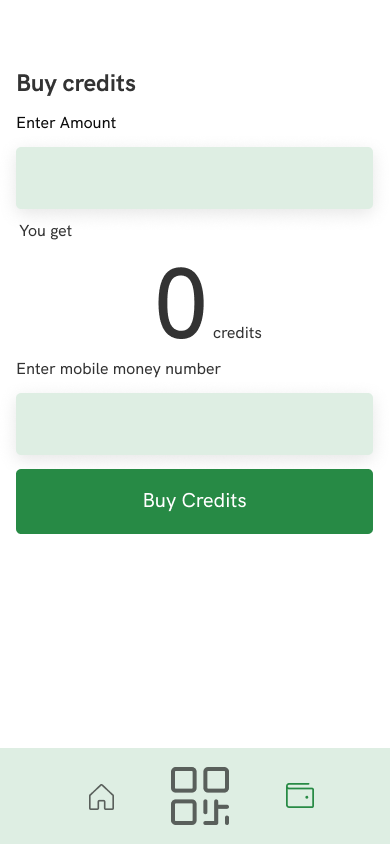
\includegraphics[scale=0.17]{images/Payments} }}%
    \subfloat[\centering]{{
\includegraphics[scale=0.17]{images/QRCode} }}%
    \caption{Home & Payment Screens of the mobile application}%
    \label{fig:example1}%
\end{figure}

\clearpage
\subsection{Silicon Pay Administrator dashboard}
THe payment gateway Silicon Pay also provides a web based dashboard which one can use to monitor transactions made through the system. The dashboard is shown below:
\begin{figure}[h]
    \begin{center}
        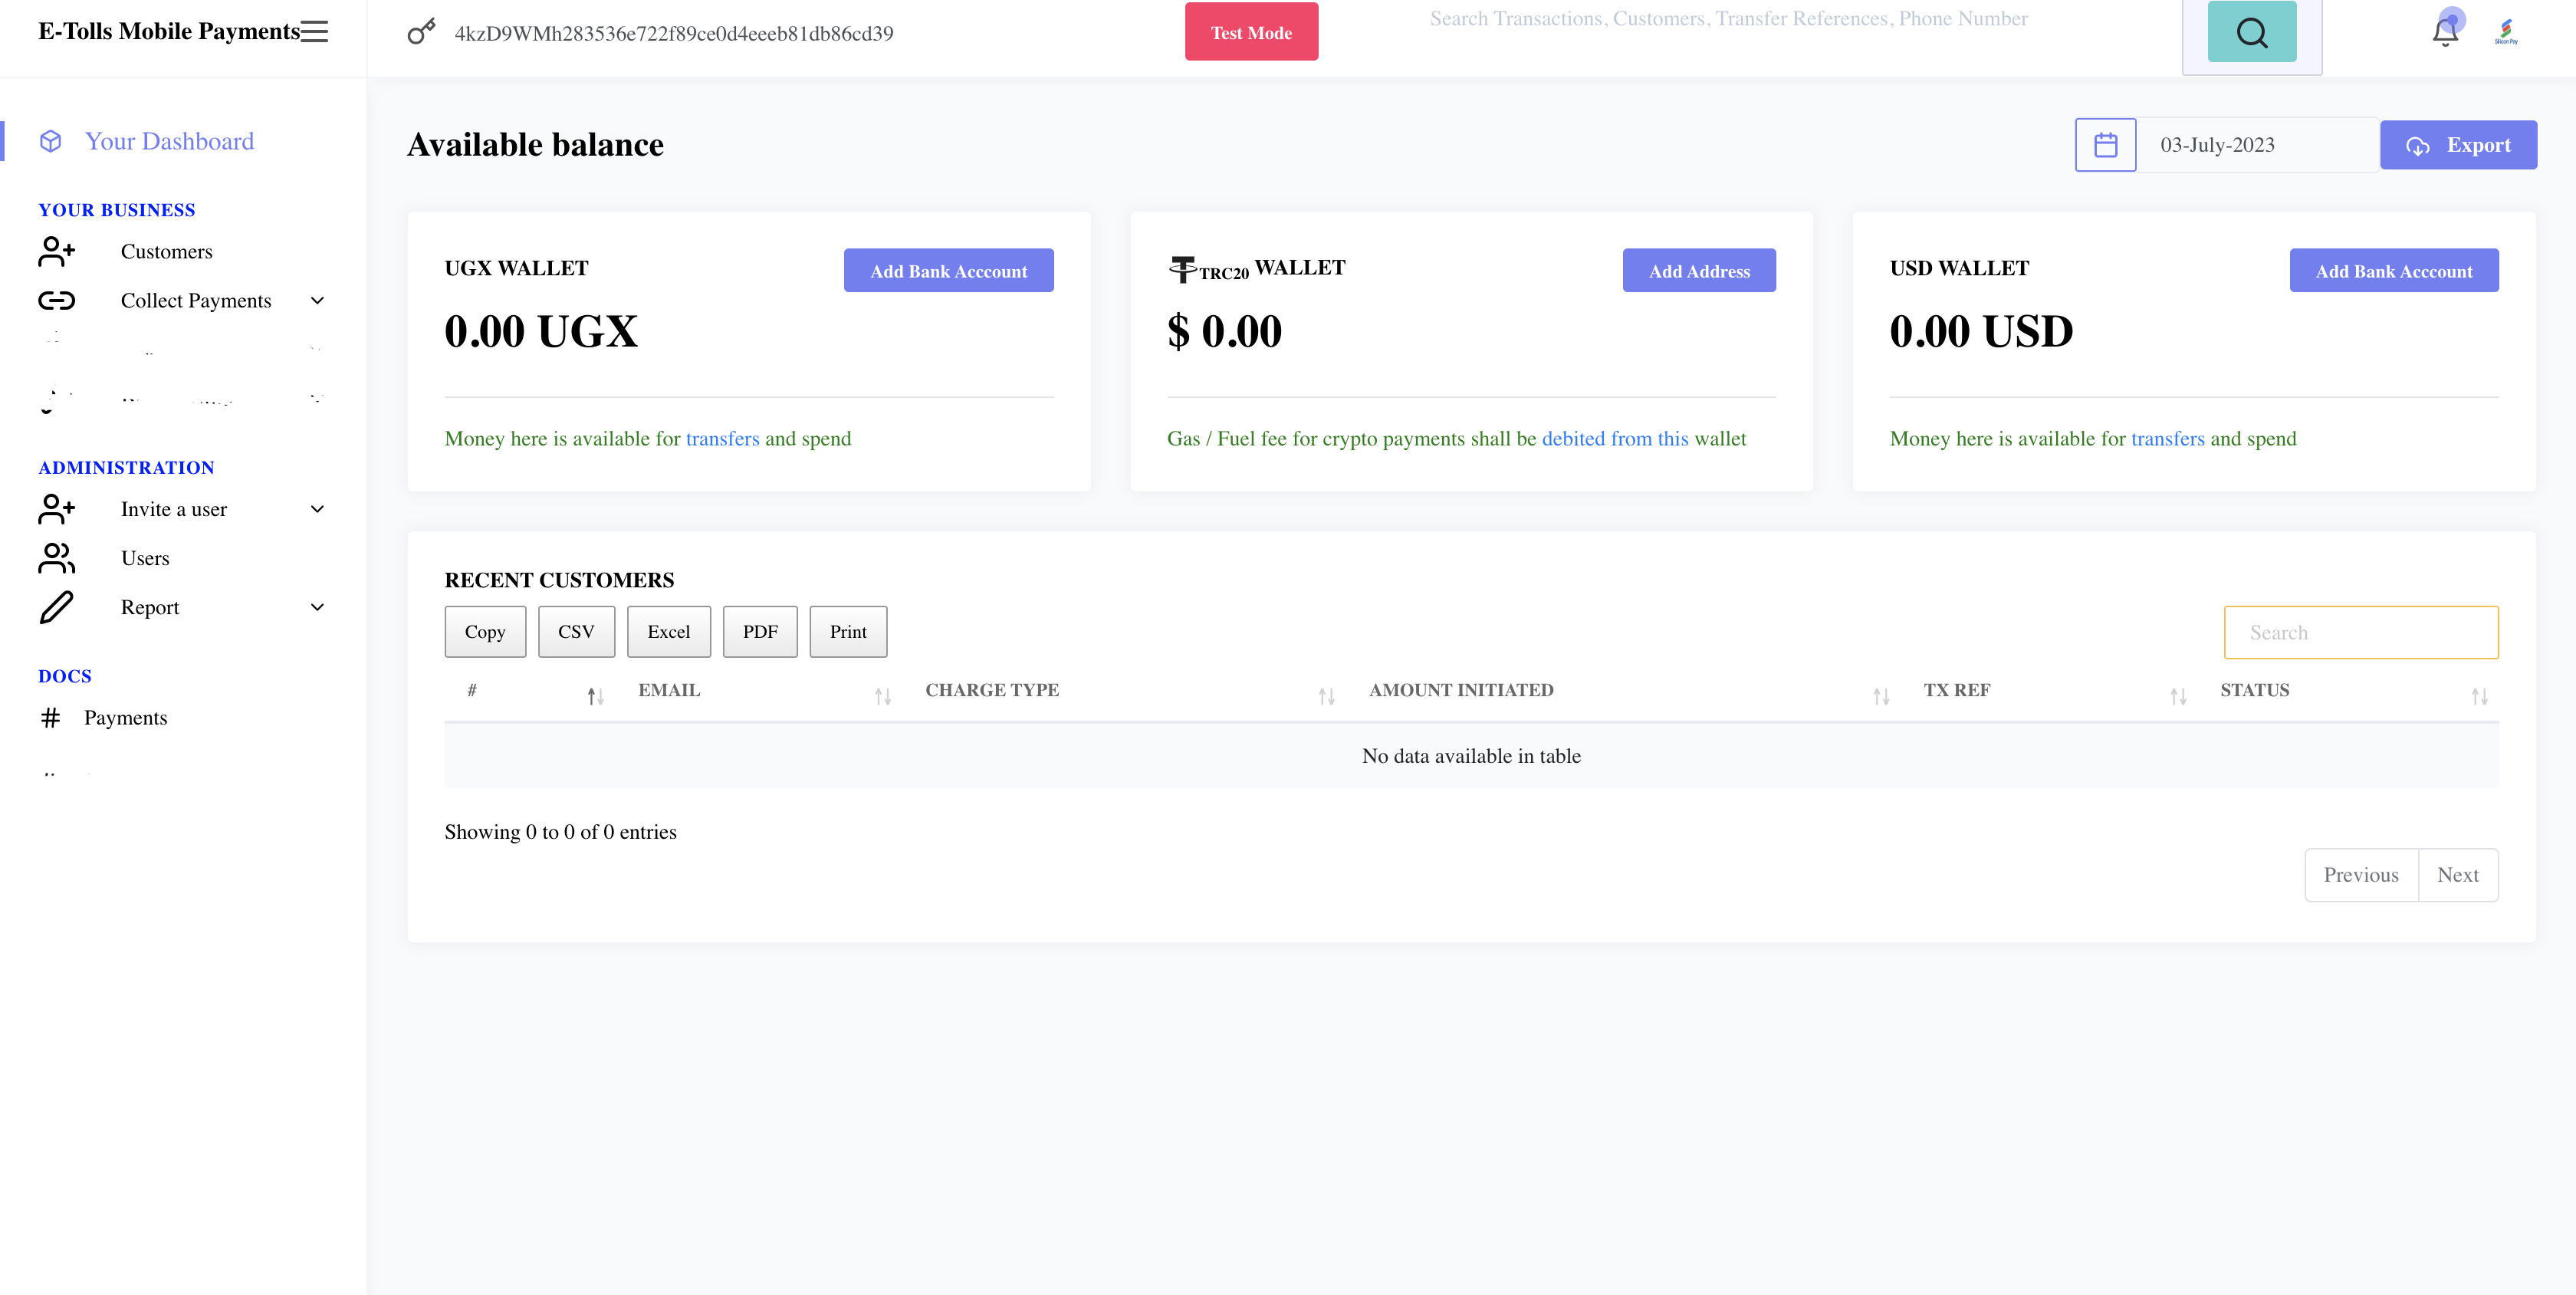
\includegraphics[scale = 0.1]{images/dashboard_1}
        \caption{Web based admin dashboard to view all transactions}
    \end{center}
\end{figure}


\begin{figure}[h]
    \begin{center}
        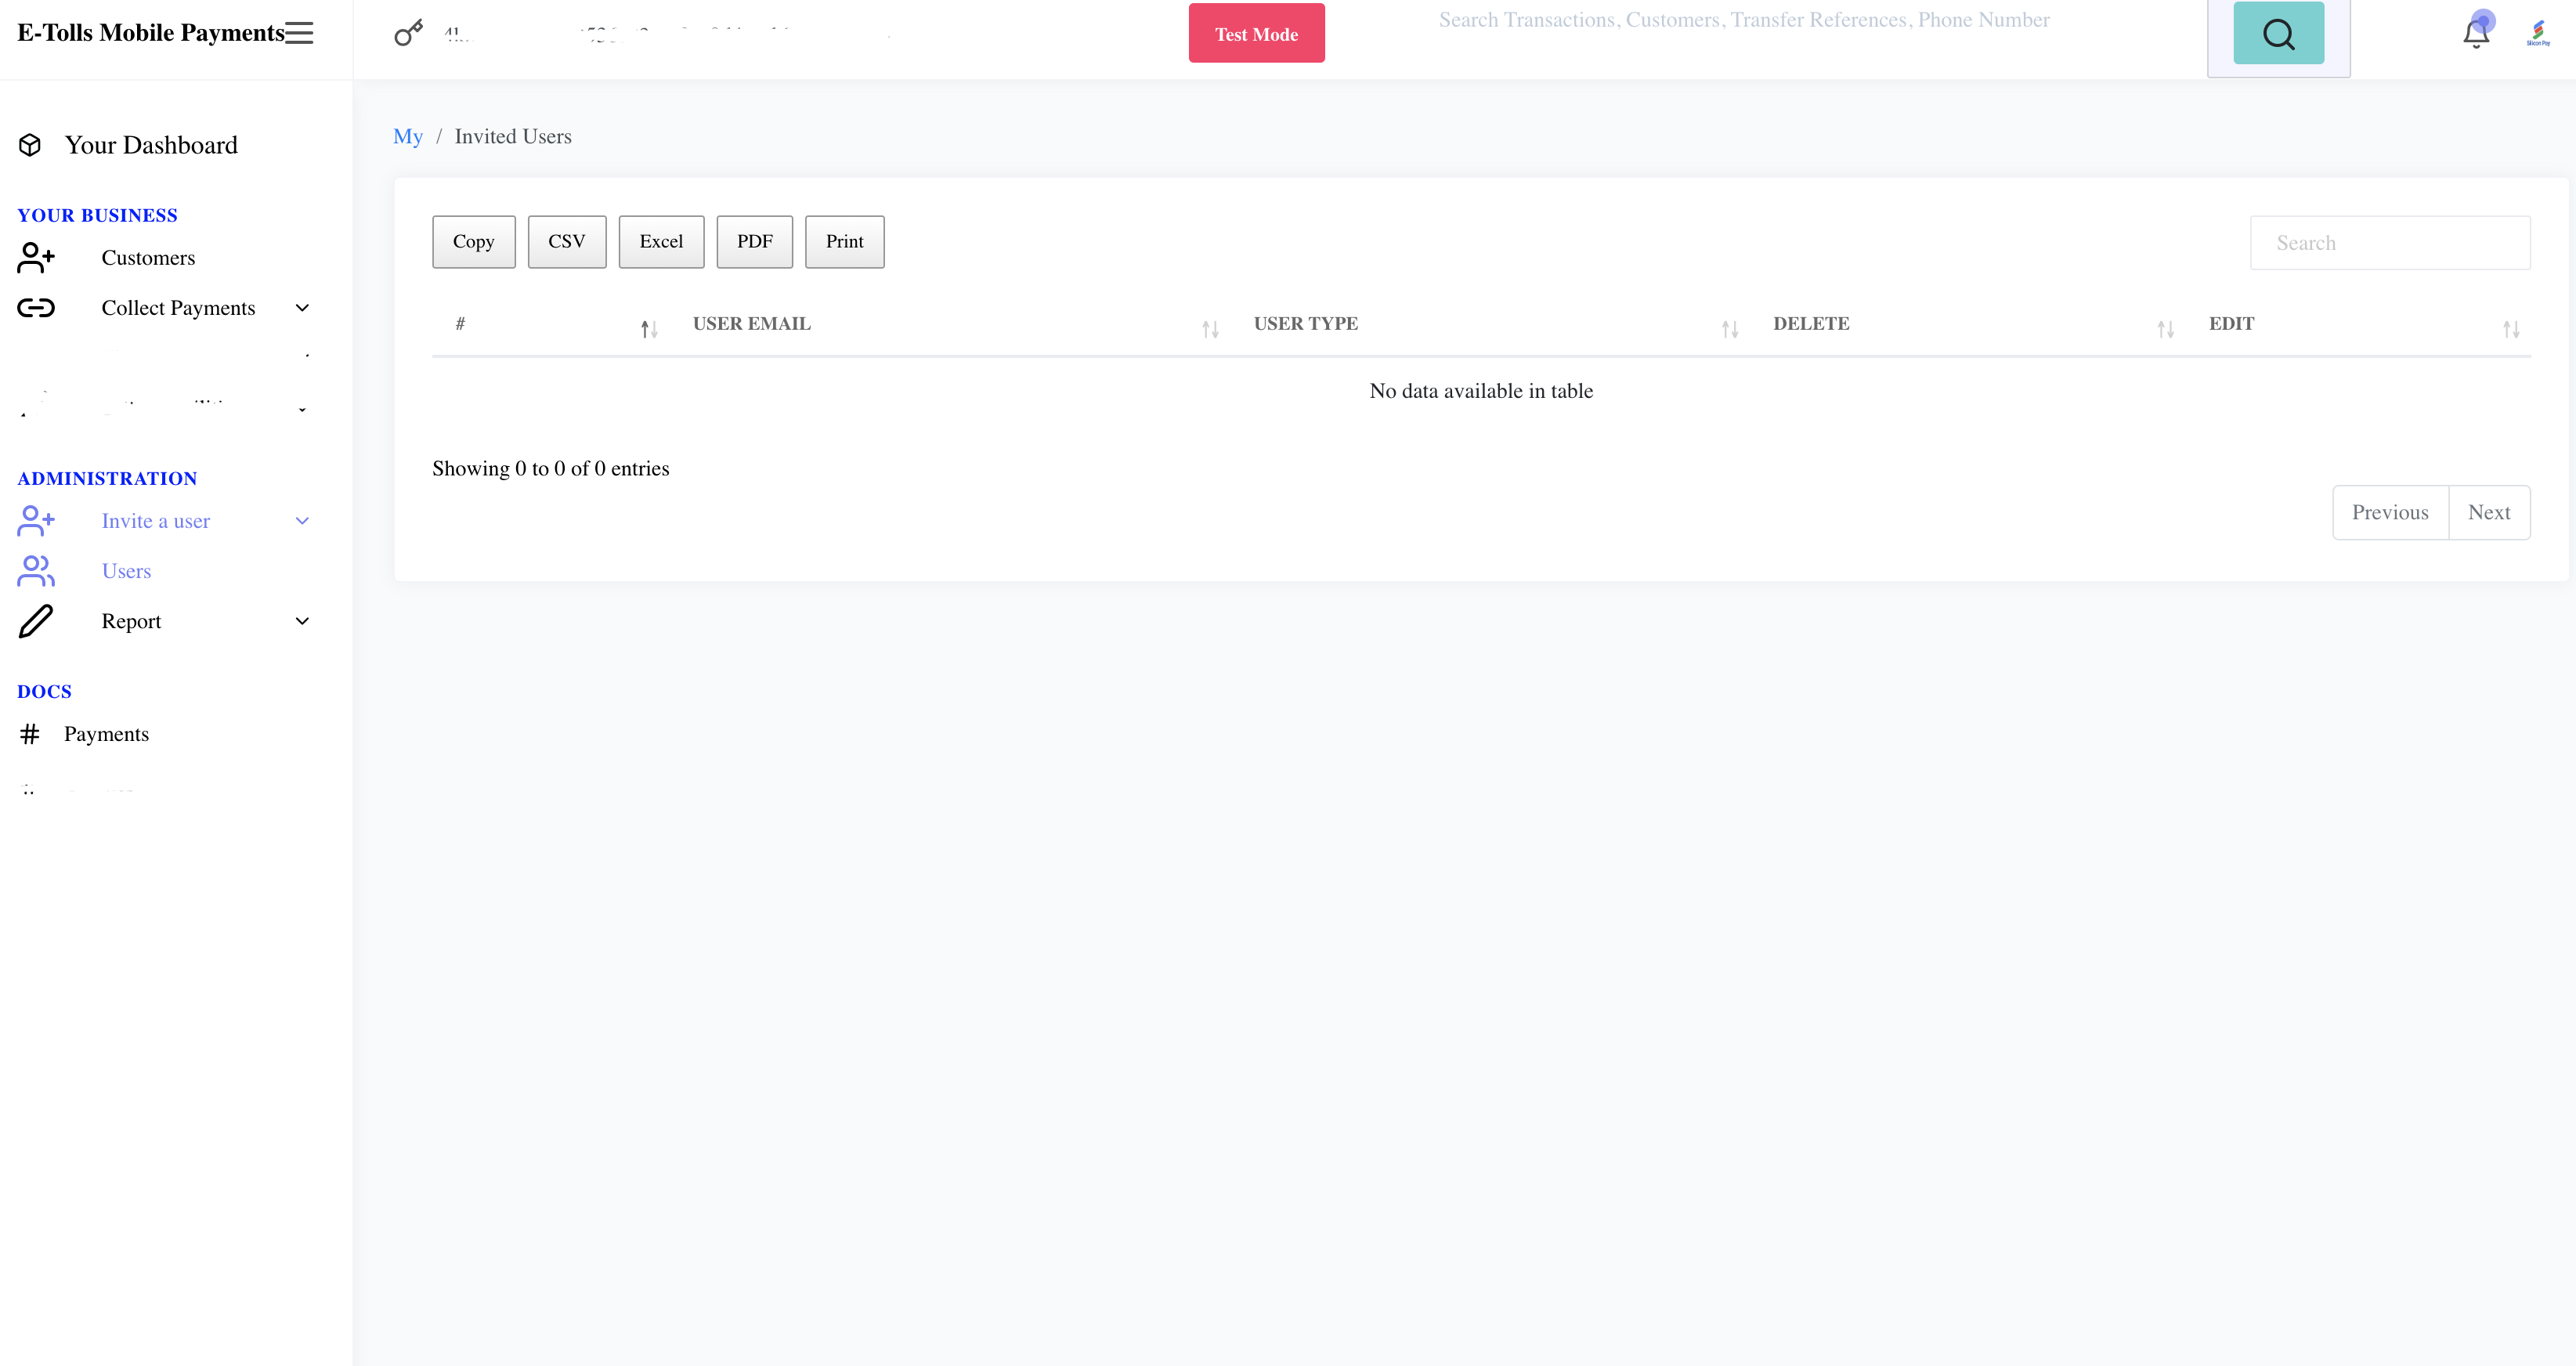
\includegraphics[scale = 0.1]{images/dashboard_2}
        \caption{Table to hold summary of customers data that can be exported as CSV/PDF}
    \end{center}
\end{figure}

\begin{figure}[h]
    \begin{center}
        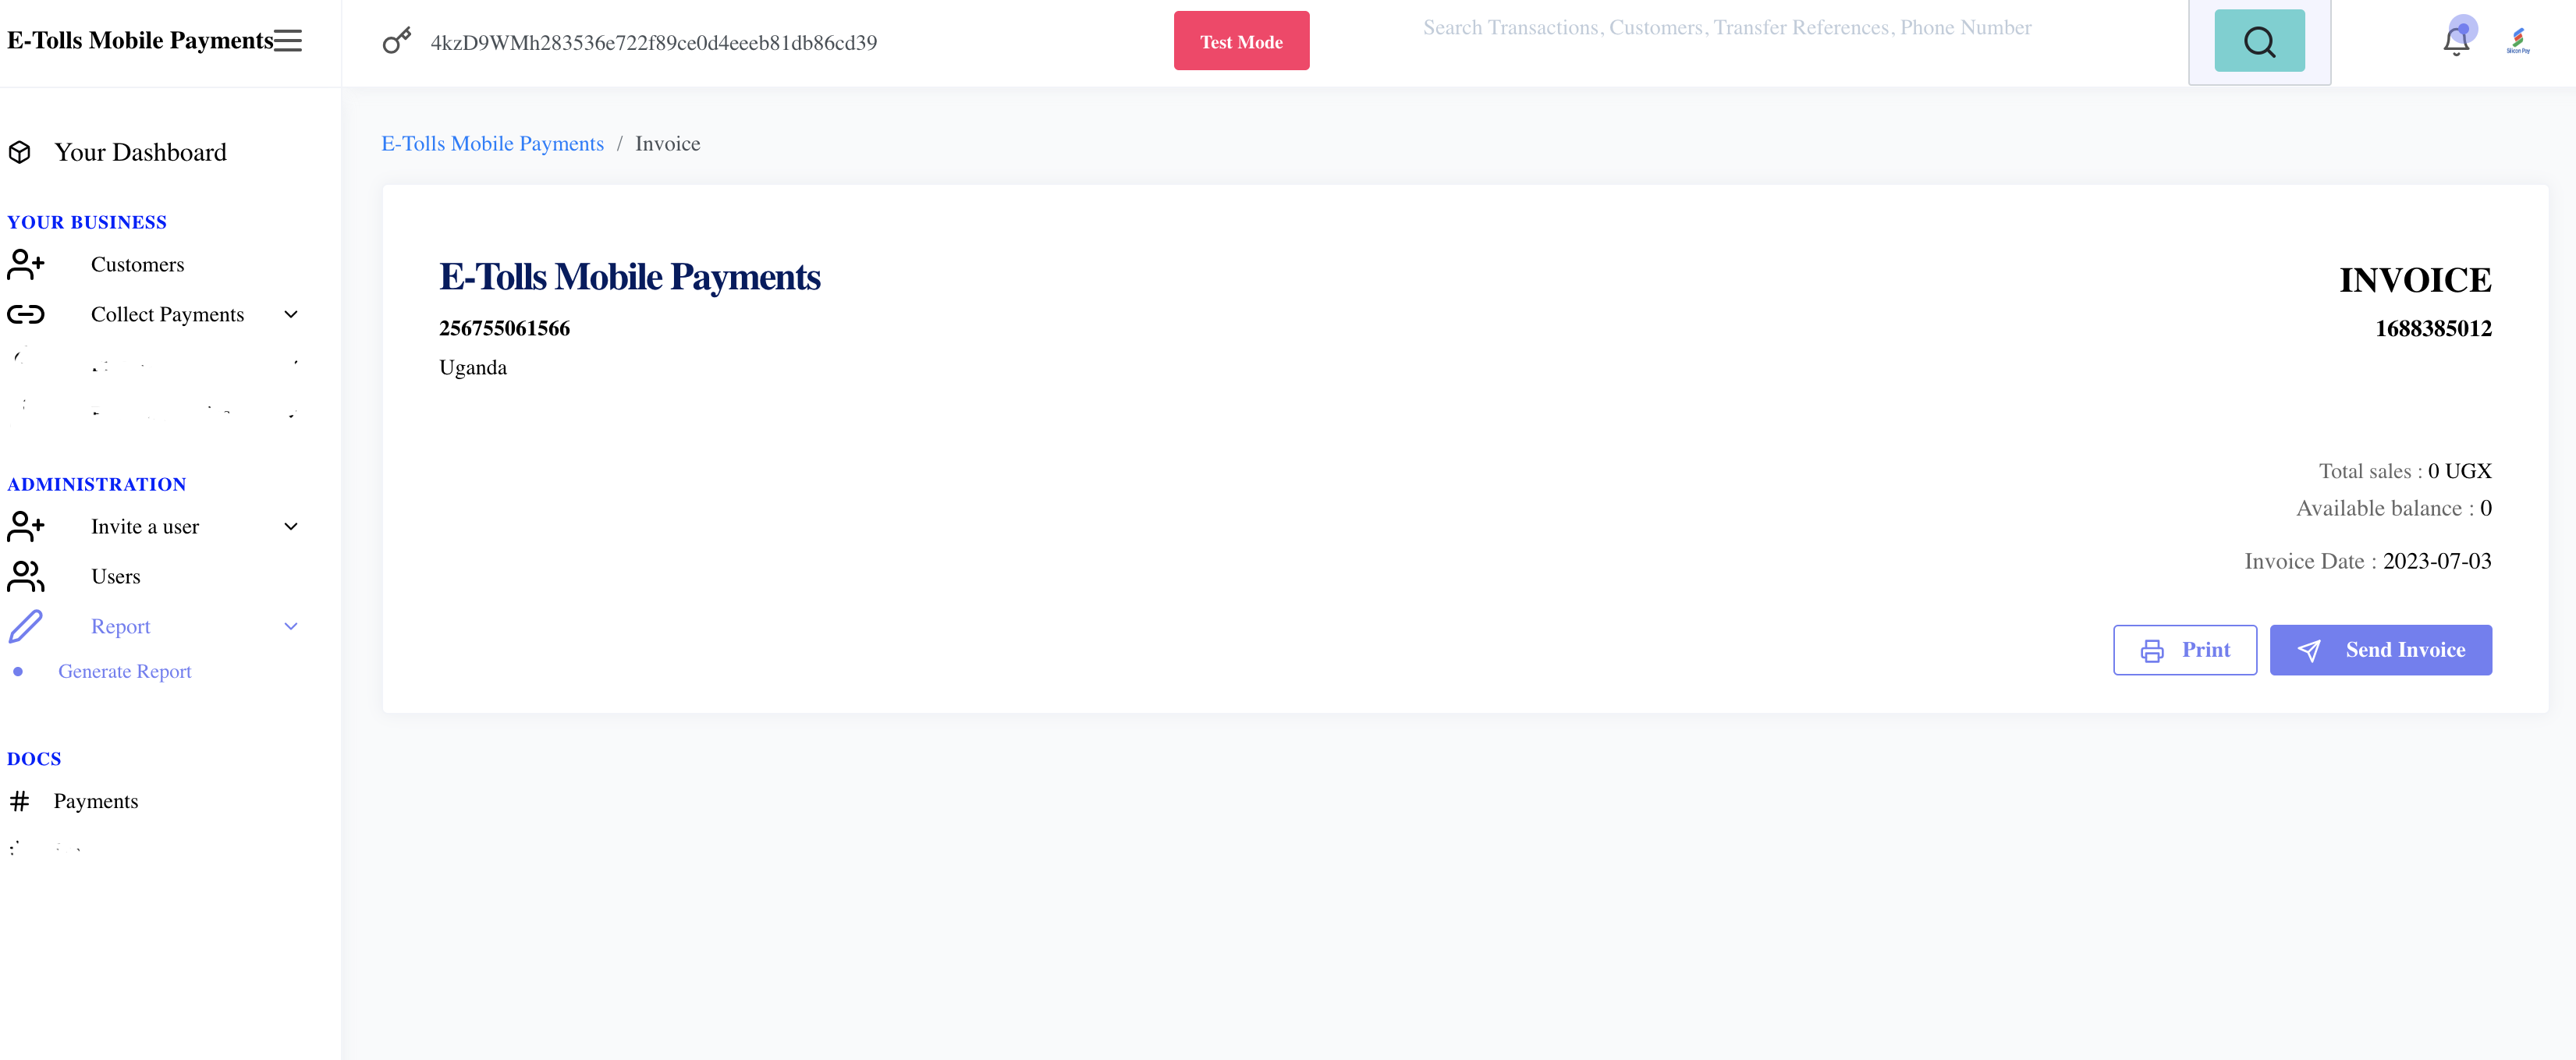
\includegraphics[scale = 0.1]{images/dashboard_3}
        \caption{ General Report of transactions made in a given period of time}
    \end{center}
\end{figure}



    \chapter{Outcomes}\label{ch:outcomes}
    The project achieve the following outcomes:
\begin{itemize}
    \item Informative results on testing and evaluating the current payment system used at toll gates in comparison to the new proposed system
    \item A well developed and operational cross-platform mobile application to enable payment of toll fees as well as verification of the payments. This application is available for both iOS and Android mobile platforms
    \item A functional embedded QR Code scanner that's able to capture QR code values and verify payments that have been made.

\end{itemize}


\section{Project Gaps and Future Works}
Currently, implementation of the project is limited to the university scope and only accounts for users with smartphones with iOS and Android Operating Systems.

\begin{figure}
    \begin{center}
        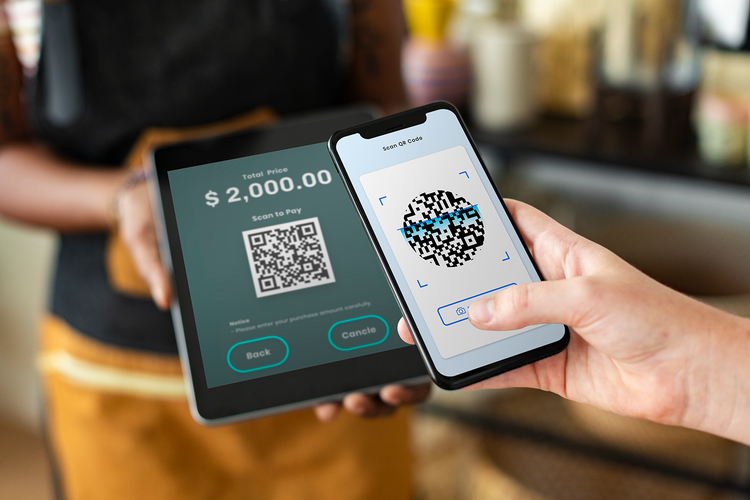
\includegraphics[scale = 1.3]{images/qr}
        \caption{The system payment is currently limited to smartphones. In future, the project could be improved to support other phones}
    \end{center}
\end{figure}
This project can easily be scaled to various places such as malls and hospitals, and extended to account for non-smartphone users.


\clearpage
\bibliographystyle{IEEEtran}
\bibliography{references}
\begin{appendices}
    \textbf{Interview Questions: Motorist}
    \begin{itemize}
        \item What are some of the challenges you have faced using Makerere's toll gates?
        \item Describe the process of payment for toll fee at the ticket stations.
        \item How many times do you use the toll gate in a day?
        \item How much do you typically spend on toll gates?
        \item Do you often find queues at the toll gates?
        \item If you do, how often does this happen and at what times of the day?
    \end{itemize}

    \textbf{Interview Questions: Toll Operator}
    \begin{itemize}
        \item How many vehicles use this gate?
        \item What challenges do you normally face when using these gates?
        \item Do you believe cashless payments would ease your organisation's work?
    \end{itemize}


    \begin{figure}
        \begin{center}
            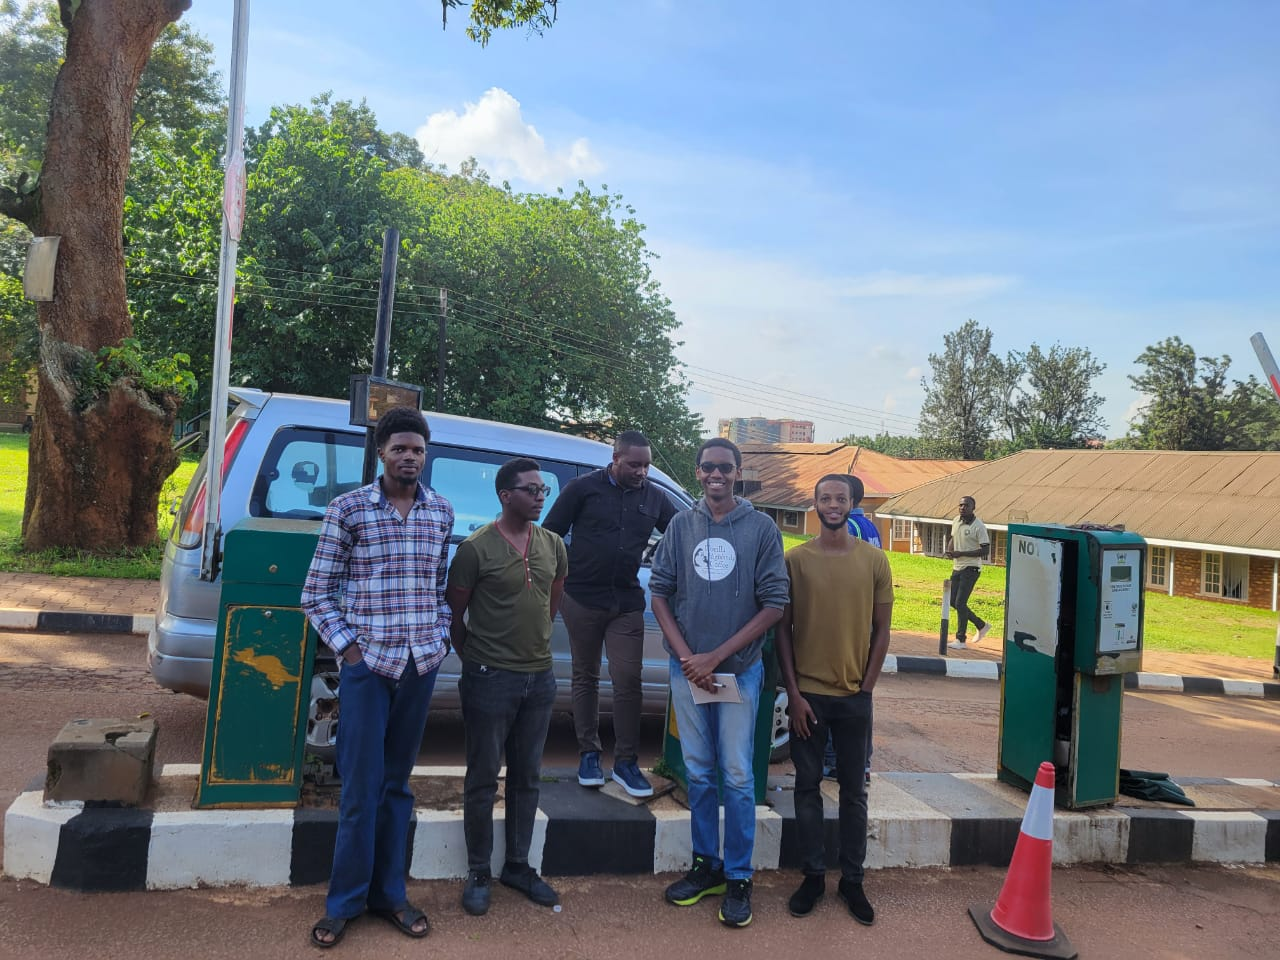
\includegraphics[scale = 0.3]{images/rizz.jpeg}
            \caption{The team members of the project conducting in person interviews with motorists and the project manager at the toll gate}
        \end{center}
    \end{figure}
\end{appendices}
\end{document}

